\documentclass[12pt,oneside,english,parskip=full,headings=small]{scrbook}

\usepackage{lmodern}
\usepackage{mathtools}
\usepackage{amsfonts}

\usepackage[a4paper]{geometry}
\geometry{verbose,tmargin=2.5cm,bmargin=2.5cm,lmargin=3.5cm,rmargin=2.5cm,headsep=0.5cm,footskip=1cm}
\usepackage{fancyhdr}
\pagestyle{fancy}

\setcounter{secnumdepth}{2}
\setcounter{tocdepth}{2}

% Generate PDF links for ToC, cite, ref, etc.
\usepackage{hyperref}

% This somehow takes advantage of pdftex features and magically make the document typeset nicer,
% for example it's managed to resolve an underfull hbox warning on its own.
\usepackage{microtype}

% To get nice numbered algorithm floats
\usepackage{algorithm}
% To actually typeset algorithms
\usepackage{algpseudocode}
% \LineComment command to make comments that are not right-aligned
\algnewcommand{\LineComment}[1]{\State \(\triangleright\) #1}

% Theorem styles
\usepackage{amsthm}

\usepackage{graphicx}
\usepackage[outdir=./out/]{epstopdf}
\graphicspath{ {./images/} }
\usepackage{subcaption}

\setlength{\parskip}{1ex}
\setlength{\parindent}{1.0cm}

% The following commands set the page numbers on the top right
% except in the beginning of chapters
% using fancyhdr package (page layout>heading style->fancy)
\lhead{}
\chead{}
\rhead{\thepage}
\lfoot{}
\cfoot{}
\rfoot{}
\renewcommand{\headrulewidth}{0pt}

% Prevent single first or last lines of a paragraph appearing alone at the top or bottom
% of a page.
\clubpenalty=10000
\widowpenalty=10000

% We get a bunch of underfull hboxes is the references, which seem hard to impossible to fix nicely,
% so this silences them for now so they're not spamming the output.
% TODO: Before actual submission, turn this off and try and fix any underfull hbox reported. If some
% can't be fixed, that's not big deal either.
\hbadness 10000

% This declares \abs and \norm commands
\DeclarePairedDelimiter\abs{\lvert}{\rvert}%
\DeclarePairedDelimiter\norm{\lVert}{\rVert}%

% Swap the definition of \abs* and \norm*, so that \abs
% and \norm resizes the size of the brackets, and the 
% starred version does not.
\makeatletter
\let\oldabs\abs
\def\abs{\@ifstar{\oldabs}{\oldabs*}}
%
\let\oldnorm\norm
\def\norm{\@ifstar{\oldnorm}{\oldnorm*}}
\makeatother

\newcommand{\todo}[1]{\paragraph{TODO} #1}

% Number definitions, theorems, and lemmas with a single counter.
\newtheorem{theorem}{Theorem}[section]
\newtheorem{lemma}[theorem]{Lemma}
\theoremstyle{definition}
\newtheorem{definition}[theorem]{Definition}

\begin{document}

% Title, declaration, ...
\frontmatter

\vspace{2.5cm}


\title{\textrm{\huge{}Algorithm Engineering for Cluster Editing}\\
	\vspace{1.8cm}
}

\author{\textbf{\LARGE{}Sebastian Paarmann}\vspace{2.5cm}
	\\
	{\normalsize{}A thesis submitted in}\\
	{\normalsize{}fulfillment of the requirements for the award of
	}\\
	{\normalsize{}Bachelor of Computer Science\vspace{3.1cm}
	}\\
	{\normalsize{}}\\
	{\normalsize{}
\includegraphics[scale=0.2]{tuhh}}\\
	{\normalsize{}\vspace{3.1cm}
}}

\maketitle
\begin{center}
	$ $\thispagestyle{plain}\addcontentsline{toc}{chapter}{Declaration}\vspace{2cm}
\par\end{center}

\begin{center}
	I hereby declare that this thesis entitled \textquotedblleft Algorithm Engineering for Cluster
	Editing\textquotedblright{} is the result of my own
	research except as cited in the references. This thesis has not been
	accepted for any degree and is not concurrently submitted in candidature
	of any other degree. \vspace{2cm}
\par\end{center}

Signature$\hphantom{xte1}$:

Student$\hphantom{Date1}$: Sebastian Paarmann

Date$\hphantom{Student1}$: \vspace{4cm}

Supervisor$\hphantom{Co}\,$: Prof. Dr. Matthias Mnich\vspace{2cm}

Co-Supervisor: Dr. Jens M. Schmidt

\newpage{}

\addchap{Acknowledgment}

Some acknowledgments I still have to write at some point.

\begin{flushright}
	Sebastian Paarmann, Henstedt-Ulzburg
\par\end{flushright}

\tableofcontents
\clearpage

\mainmatter

\chapter{Introduction}

A \emph{cluster} graph, also called \emph{transitive} graph, is a graph which consists only of
disjoint cliques. In the \textsc{Cluster Editing} problem, the input is an undirected graph $G$ and
an integer $k$ greater $0$, and the question is whether the $G$ can be made into a cluster graph
using $k$ or less \emph{edge edits}. An edit is either inserting an edge or deleting an existing
one.  We also consider the \textsc{Weighted Cluster Editing} problem: The input has weights for each
edge and non-edge, which are the deletion and insertion costs respectively. The question is then
whether there is a solution with total edit costs at most $k$.

\begin{figure}[h]
	\centering

	\begin{subfigure}{0.49\textwidth}
		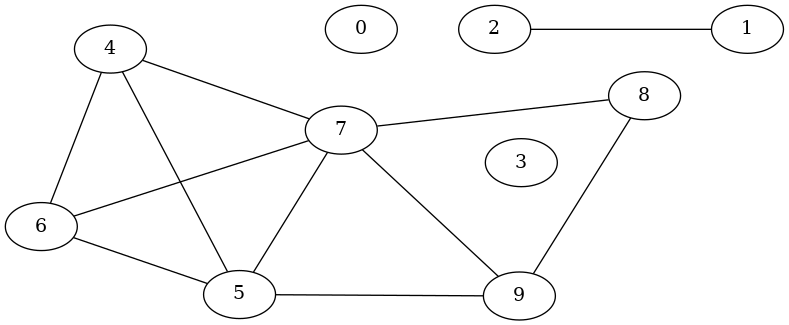
\includegraphics[width=1.0\linewidth]{exact001-input}
		\subcaption{Input graph}
	\end{subfigure}
	\begin{subfigure}{0.49\textwidth}
		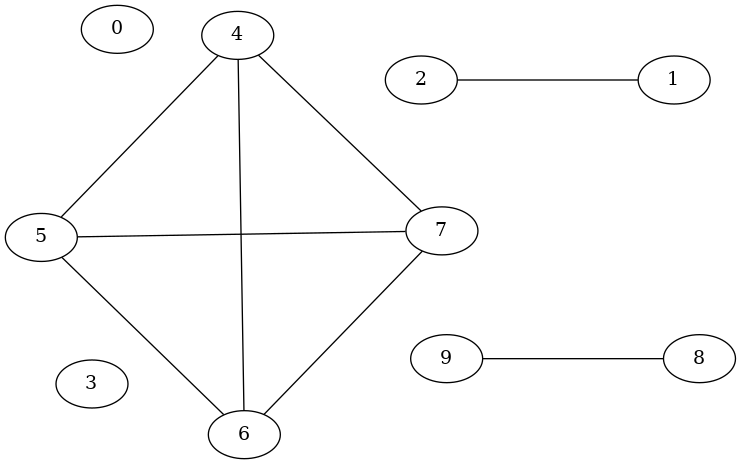
\includegraphics[width=1.0\linewidth]{exact001-output}
		\subcaption{Resulting cluster graph}
	\end{subfigure}

	\caption{First test instance of the PACE challenge}
	\label{fig:exact001}
\end{figure}

For this thesis, we have implemented a \textsc{Cluster Editing} solver as a submission to the
Parameterized Algorithms and Computational Experiments (PACE) Challenge 2021~\cite{Pace}. Among
other goals, the PACE challenge aims to result in easily available performant implementations to the
posed problems while also encouraging new theoretical developments. In the 2021 challenge, there are
three different tracks for tackling different aspects of the problem: The exact track asks to find
an optimal solution for a given graph as quickly as possible, the heuristic track asks to find a
solution that is as good as possible within a time limit, and the kernelization track asks to reduce
an input graph into a smaller equivalent instance. Our implementation is intended for the exact
track. See Figure~\ref{fig:exact001} for an example, left is the first and smallest public test
instance of the PACE challenge and right is the cluster graph resulting from an optimal solution.

\textsc{Cluster Editing} was initially introduced in the context of bioinformatics to clean data
containing measurement errors by clustering gene expression patterns~\cite{BenDor}. It has since
been applied for a variety of problems in bioinformatics, including around sequencing genes,
comparative transcriptomics, metabolic profiling in spectrometry data, and
more~\cite{BoeckerBaumbach}. As one case of the \textsc{Correlation Clustering} problem, applications
have also been found in machine learning contexts, for example to perform deduplication of
data~\cite{Bansal}.

\chapter{Preliminaries}

First, some notation used throughout this thesis: A graph $G = (V, E)$ has a vertex set $V$ and edge
set $E \subseteq \binom{V}{2}$. Graphs are simple graphs, i.e.\ they contain no self-loops or
parallel edges. We abbreviate an edge or non-edge $\{u, v\} \in \binom{V}{2}$ as $uv$. We denote the
(open) neighborhood of a vertex $v$ in $G$ as $N_G(v)$. Similarly, $N_G[v]$ is the closed
neighborhood of~$v$, i.e.\ $N_G(v) \cup \{v\}$. If it is clear which graph is meant, we may also
just write $N(v)$ and $N[v]$. A weighted graph $G$ is characterized by a weight function $s\colon
\binom{V}{2} \to \mathbb{Z}$. We consider $uv$ to be an edge if $s(uv) > 0$ and $uv$ to be a
non-edge if $s(uv) \leq 0$. For a set $U \subseteq V$, $G[U]$ is the subgraph induced by $U$ on $G$,
i.e.\ $G[U] = (U, \{ uv \in E \mid u \in U \land v \in U \})$. We write $A \Delta B$ for the
symmetric difference of two sets $A$ and $B$: $A \Delta B = (A \setminus B) \cup (B \setminus
A)$.

\todo Notation paragraph needs some cleanup; and at the end make sure this has everything relevant
that's used and nothing that isn't.

Formally the \textsc{Cluster Editing} problem can be described as follows: The input $(G, k)$
consists of a simple unweighted graph $G = (V, E)$ and parameter $k \in \mathbb{N}$. The task is to
find a cluster editing $F$ with cost less than $k$. A set $F \subseteq \binom{V}{2}$ is a cluster
editing for $G$ if the graph $(V, E \Delta F)$ is a cluster graph, i.e.\ a disjoint union of
cliques. The \emph{cost} of a cluster editing $F$ is $\abs{F}$. In the PACE challenge, we want to
solve the optimization version of this problem: The input is only a graph $G$ and the goal is to
find an optimal solution, i.e.\ a solution with the smallest amount of edits possible.

In the \textsc{Weighted Cluster Editing} problem, instead of the unweighted graph, the input
contains a weighted graph encoded by the weight function $s\colon \binom{V}{2} \to \mathbb{Z}$. The
cost of a cluster editing $F$ is then $\sum_{e \in F} \abs{s(e)}$. Our solver is intended for the
unweighted problem, as required by the PACE challenge, but it internally converts its input into a
weighted problem instance for more efficient solving. It could be adapted to take a weighted
instance with minimal modifications. One can also consider the weighted problem with real-valued
weights, but we will not do so further here.

\textsc{Cluster Editing} is NP-complete~\cite{ShamirModifications}, so there is no polynomial time
algorithm for solving it (unless P = NP). It is however \emph{fixed-parameter tractable}.
Fixed-parameter tractability (FPT) is a concept from parameterized complexity theory. A problem is
called fixed-parameter tractable if there is an algorithm to solve it in time $f(k) * n^c$, where
$n$ is the size of the input, $k$ is some additional parameter, $c$ is a constant independent of
both $n$ and $k$, and $f$ is some computable function. In general there can be many different
parameters $k$ for a single problem, for example some measure of the complexity of the input (e.g.\
maximum degree in a graph) or a limit on the size of the solution. In this way the exponential
increase in runtime can be contained in the parameter, instead of the algorithm scaling
exponentially with the input size. More detailed information can be found e.g.\ in the book of Cygan
et al.~\cite{ParameterizedAlgorithms}. In our case $k$ describes the maximum amount of edits, i.e.\
the maximum size of the solution, and $n$ is $\abs{G}$. To solve the optimization problem that is
required by the PACE challenge with a parameterized FPT algorithm, we simply execute the algorithm
in a loop starting with $k = 1$ and increase $k$ until we find a solution.

We make use of some important techniques from the field of parameterized algorithms, mainly
\emph{kernels} and data reduction rules, and \emph{bounded search trees}. Data reduction rules take
as input a problem instance, including a parameter, and produce a second instance that is equivalent
to the input one. Two instances are equivalent if there is a solution for the second if and only if
there is also a solution for the first instance. Clearly the goal is to return an instance that is
in some way \emph{easier}, for example by making the input smaller or reducing the parameter. We
describe the various reduction rules used in our algorithm in section~\ref{sec:reduction}. A
kernel is a preprocessing algorithm which gives an upper bound on the size of the returned instance
in terms of the input parameter $k$. Kernels are often implemented in terms of multiple reduction
rules that are repeatedly applied.

Apart from the reduction rules, the general shape of the algorithm we implement is that of a bounded
search tree algorithm, also called a branching algorithm. This is essentially the idea of
backtracking: The algorithm takes some decision regarding the solution (e.g.\ adding or removing an
edge) and then recursively executes on the resulting instance. If that recursive call does not yield
a solution, a different decision is taken instead and the procedure repeated. If it can be
guaranteed that some sequence of decisions will lead to a solution if one exists, this kind of
algorithm correctly solves the problem. It can be viewed as recursively moving through a search tree
where each ``decision point'' is a node. As the name says, the search tree should also be bounded:
There should be a limit on the amount of branches taken in each node as well as a guarantee that
after each decision the instance is substantially simpler such that we will eventually reach a leaf
node where the solution (or its non-existence) is trivial.

\begin{figure}[h]
	\centering
	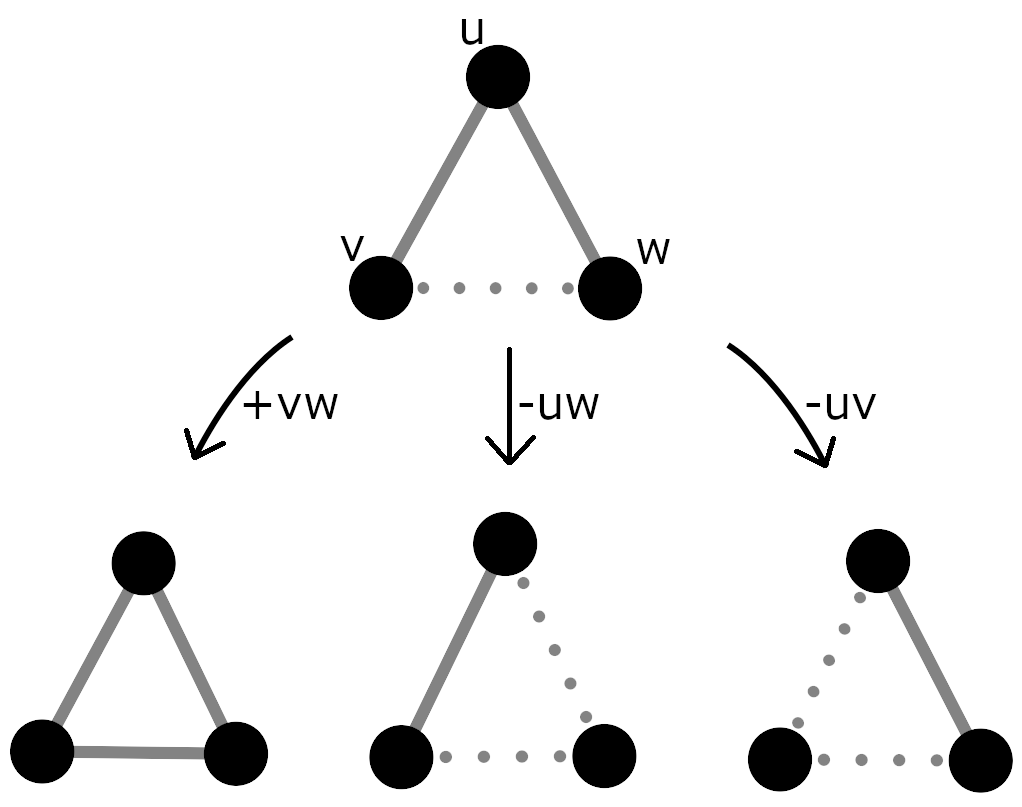
\includegraphics[scale=0.5]{conflicts}
	\caption{A conflict $v u w$ and three ways to resolve it.}
	\label{fig:conflicts}
\end{figure}

A central observation regarding the \textsc{Cluster Editing} problem is that a graph $G = (V, E)$ is
a cluster graph if and only if there is no \emph{conflict triple} in the graph. Three vertices $v,
u, w \in V$ form a conflict triple if $uv, uw \in E, vw \notin E$, i.e.\ the vertices form an
induced $P_3$. This leads to a very simple search tree algorithm: The problem can be solved by
recursively searching for a conflict triple and branching into three cases: Add $vw$, remove $uv$,
or remove $uw$. These are the only ways of resolving a conflict, and once there are no more
conflicts, a solution can be returned. Looking at our criteria for a bounded search tree from above,
this has a limit on the branches per node, exactly three. And for each branch we perform an edit on
the graph and thus reduce $k$ by 1, limiting the depth of the search. This algorithm gives a search
tree of size $O(3^k)$, though we will see in the next sections that more efficient trees are
possible. The basic idea of this branching strategy is illustrated in Figure~\ref{fig:conflicts}.

\chapter{Previous Work}

%todo Maybe change listing of 3 authors to et al.?

Clustering problems in general have a very long history, so we will focus only on the specific
\textsc{Cluster Editing} problem as formulated above. In 1999, Ben-Dor, Shamir, and
Yakhini~\cite{BenDor} introduced the unweighted problem in order to perform clustering on gene
expression patterns. They provided a stochastic model for the corruption of the true clustering
introduced by measurements and present an $O(n^2 \log(n)^c)$ algorithm that reconstructs the true
clustering with high probability, as well as a heuristic approach based on a similar idea. Many
other approaches for clustering gene expression data had been proposed and investigated already at
this time, see \cite{ShamirOverview} for an overview from 2001.

Shamir, Sharan, and Tsur~\cite{ShamirModifications} investigated \textsc{Cluster Editing} as well as
the related \textsc{Cluster Completion} (only edge insertions allowed) and \textsc{Cluster Deletion}
(only edge deletions allowed) problems further. They showed that \textsc{Cluster Completion} can be
solved in polynomial time, \textsc{Cluster Deletion} is NP-hard to approximate to within some
constant factor, and, most relevant for us, \textsc{Cluster Editing} is NP-complete.  Additionally
they also considered variants of the problems with a fixed number of clusters as input, which we
will not further discuss here. Gramm et al.~\cite{Gramm} also mention that the NP-completeness of
\textsc{Cluster Editing} can already be derived from the work of Křivánek and
Morávek~\cite{Krivanek}, published in 1986.

Bansal, Blum, and Chawla independently researched a group of problems they call \textsc{Correlation
Clustering}~\cite{Bansal}. In this formulation, ``minimizing disagreements'' between the input
labelling and the output clustering is equivalent to the unweighted \textsc{Cluster Editing}
problem, which they give a constant-factor approximation for. This result was improved on in 2005 by
Charikar, Guruswami, and Wirth~\cite{Charikar}, who show the problem to be APX-hard and give an
approximation with a constant factor of 4.

In 2003 Gramm et al.~\cite{Gramm} gave initial results regarding fixed-parameter approaches for
\textsc{Cluster Editing} specifically. Before that, Cai~\cite{Cai} investigated fixed-parameter
tractability of graph modification problems characterized by forbidden subgraphs in a more general
sense, the results of which imply an $O(k^3 * \abs{G}^4)$ algorithm for \textsc{Cluster Editing}.
Gramm et al.\ gave an $O(k^3)$ kernel for the problem, as well as a straightforward $O(k^3 + n^3)$
fixed-parameter algorithm. Additionally they show a more advanced branching strategy that improves
the search tree size to $O(2.27^k)$, leading to an $O(2.27^k + n^3)$ algorithm.  This approach was
implemented in practice for the first time and empirically compared to an LP-based solver by Dehne
et al.\ in 2006~\cite{Dehne}. They find that the $O(2.27^k)$ is indeed faster in practice than the
simpler $O(k^3)$ branching. Additionally Gramm et al.\ also presented a method for generating search
tree algorithms in a computer-assisted fashion and used it to show a $O(1.92^k)$ search
tree~\cite{AutomatedSearchTree}.

Another avenue of research was started in 2007 by Rahmann et al.~\cite{Rahmann}. This introduced the
first fixed-parameter algorithm for the weighted version of the problem, along with several data
reduction rules to speed it up. They also introduced two heuristic algorithms.

Building on this, Böcker et al.\ published several papers in 2008. They introduce a variant of the
refined branching strategy of Gramm et al.~\cite{Gramm} for the weighted problem, resulting in an
$O(2.42^k)$ algorithm~\cite{AnApproach}. Most importantly, this is the first paper to introduce
merging two vertices, which is an operation only possible on the weighted problem. As a result, with
merging, Böcker et al.\ find the simpler $O(3^k)$ branching faster in practice than the refined
branching strategy, largely due to the significant effect of merging. Merging is also the basis for
a very simple $O(2^k)$ branching algorithm~\cite{GoingWeighted} which means the fastest practical
approach to solving the unweighted problem is now to transform it into a weighted instance and solve
that.  The paper also immediately improves upon this with an $O(1.82^k)$ algorithm that is achieved
by more carefully choosing which edge to branch on. This beats even the previous best theoretical
runtime for the unweighted problem of $O(1.92^k)$. Lastly, Böcker et al.\ perform practical
experiments with these algorithms~\cite{ExactAlgos}, comparing them with a cut-and-branch based ILP
implementation.  They find both approaches to be competitive, with different performance
characteristics. Notably, good data reduction rules make the FPT approach feasible even for graphs
that require several thousand edge modifications, despite the worst-case running times.

This basic approach was improved further by Böcker and Damaschke. First, a theorem introduced by
Damaschke~\cite{BoundedDegree} concerning the structure of graphs in which no edge is part of three
conflict triples, is used to improve the algorithm to $O(1.76^k)$~\cite{EvenFaster}. Then zero-edges
(which will be discussed in more detail later) can be used to show additional structural properties,
allowing even more efficient branching for an $O(1.62^k)$ search tree~\cite{GoldenRatio}.

In parallel multiple problem kernels for \textsc{Cluster Editing} have also been developed. Note
that we discuss them here separately only to make it easier to follow, in practice the work on
kernels is often what makes the better algorithms possible: Better reduction rules introduced as
part of a kernel allow constructing and proving a faster search tree algorithm. In fact, these are
often developed as a single work. Such it is for the first kernel given by Gramm et al.~\cite{Gramm},
which has at most $2k^2 + k$ vertices and can be computed in $O(n^3)$ time.

Protti, da Silva, and Szwarcfiter~\cite{Protti} gave a kernel with at most $2k^2 + 4k$
vertices, slightly worse than that off Gramm et al.\ but still $O(k^2)$. It is based on the modular
decomposition of a graph and has the advantage of only requiring running time $O(n + m)$. In 2007,
Fellows et al.\ introduced a ``crown-type structural reduction rule''~\cite{Fellows} and show it
can be used to construct a kernel with $6k$ vertices that can be computed in polynomial time.

Based on both the ideas of the crown-type reduction and the concept of \emph{critical cliques},
which had already been used for good effect in fixed-parameter approaches to other problems,
Guo~\cite{Guo} presented first another $6k$ kernel with $O(n^3)$ runtime and immediately improved
this to a kernel with at most $4k$ vertices computable in $O(nm^2)$ time. In 2011, Chen and
Meng~\cite{ChenMeng} combined the critical cliques concept with the notion of an \emph{editing
degree} of a vertex to give a $2k$ kernel which runs in $O(nm)$ time.

In 2015 Hartung and Hoos developed and published a \textsc{Cluster Editing} solver that outperforms
previous implementations~\cite{HartungHoos}. They use the \emph{Programming by Optimization}
paradigm, using automated methods to optimize algorithm behavior and parameter choice and guide
further manual optimization effort based on empirical tests, to create an implementation that relies
mainly on a reduction technique that is worse than newer ones from a theoretical point of view but
is able to produce significant runtime improvements in practice on their varied test data.

Lastly, there are also \emph{integer linear programming} (ILP) formulations of the problem and
associated solvers which we have already mentioned in relation to other work above. As we
implemented only a bounded search tree algorithm, we do not go into further detail regarding these
approaches but note the early work of Grötschel and Wakabayashi~\cite{CuttingPlane} and the modern
$\mathsf{yokisho}$ solver~\cite{yokisho} that combines an ILP solver with data reduction rules.

\chapter{Our Implementation}

In this section we will describe the implementation of our solver in some detail. It is based on
many techniques introduced by the papers mentioned above. Those are only briefly summarized there
but we will give more detailed information about those we have implemented here.

There are 4 parts to this section: We start off by describing the high-level structure of the
solver, followed by a more in-depth look at the two basic modifying operations that are performed on
the graph during execution of the algorithm. Next, we describe the reduction rules used, and finally
some details on the practical implementation of the described algorithm, e.g.\ used data structures.

\section{High-Level Overview}

The solver consists of two main parts: The solver function, Algorithm~\ref{alg:solver}, that
performs interleaved reduction and the branching strategy, calling itself recursively; and a
\emph{driver}, Algorithm~\ref{alg:driver} that splits the input graph into its connected components,
performs some initial reduction and conversion to a weighted instance, and then calls the recursive
solver function with increasing parameter $k$ until a solution is found. 

As mentioned before, we implement a bounded search tree approach with multiple data reduction
techniques. We currently use a very simple branching strategy: We take a conflict triple $v, u, w$
and branch into two cases, merging $uv$ and forbidding $uv$. These operations will be described in
more detail in the next section. This strategy was introduced by Böcker et al.~\cite{GoingWeighted}
and shown to lead to a search tree size of $O(2.62^k)$. Böcker et al.\ also introduced more advanced
branching strategies, with even smaller search trees which would also like to implement but have not
so far due to time constraints.

The reductions are split into several categories. There is the initial step of taking an
unweighted instance and turning it into a reduced weighted instance. A set of parameter-independent
reduction rules can also be applied directly after this, before the main search-tree algorithm.
These parameter-independent rules are also applied interleaved during the search. And finally, any
reductions that depend on having a maximum cost parameter $k$ can be applied only once the search
has started.

During the recursive search, we must track the current graph, which is modified for each recursive
step, the current value for $k$ as well as the set of edits done so far in the current branch.
Because we modify the graph not just by inserting and deleting edges in the course of the algorithm,
but also by merging vertices (which effectively removes a vertex; see below for details), we also
need to keep track of which vertices in the current graph correspond to which vertices of the
original graph. One can either keep tracking edits throughout the branching search in terms of the
original graph, or reconstruct the edit set at the end based on the final graph and the information
about how vertices correspond. Theoretically the latter is more optimal in terms of runtime because
it only needs to do some work once the solution has been found, while the former approach has a
slight overhead while searching. Our testing has indicated the difference is negligible however and
we currently implement the former approach. What this means in practice is that if we perform an
edit on the graph, we also look up which original vertices correspond to the two vertices involved
and record edits for each possible pair.

\begin{algorithm}[h]
\caption{Driver}
\label{alg:driver}
\begin{algorithmic}

\Function{ComputeOptimalClusterEditing}{$G: Graph$}
	\State $edits \gets \emptyset$
	\ForAll{$comp \in \Call{Components}{G}$}
		\State $instance \gets \Call{MakeWeightedInstance}{comp}$
		\State ($instance, lb1) \gets \Call{InitialReduction}{instance}$
		\State $lb2 \gets \Call{LowerBound}{instance}$
		\State $k \gets \Call{Max}{lb1, lb2}$
		\Repeat
			\State $solution = \Call{SolveClusterEditing}{instance, k, \emptyset}$
			\State $k \gets k + 1$
		\Until{$solution \neq \emptyset$}

		\State $edits \gets edits \cup solution$
	\EndFor
	\State \Return $edits$
\EndFunction

\end{algorithmic}
\end{algorithm}

\begin{algorithm}[h]
\caption{Recursive Solver}
\label{alg:solver}
\begin{algorithmic}

\Function{SolveClusterEditing}{$instance, k, edits$}
	\If{$k < 0 \lor k < \Call{LowerBound}{instance}$}
		\State \Return $\emptyset$
	\EndIf

	\State $\Call{Reduction}{instance, k, edits}$

	\If{$k < 0 \lor k < \Call{LowerBound}{instance}$}
		\State \Return $\emptyset$
	\EndIf

	\If{$\neg \Call{HasConflictTriple}{instance}$}
		\State \Return $edits$
	\EndIf

	\State $(v, u, w) \gets \Call{GetConflictTriple}{instance}$
	\\
	\LineComment Branch 1: Forbid $uv$
	\State $delInstance \gets \Call{Clone}{instance}$
	\State $delK \gets k$
	\State $delEdits \gets \Call{ForbidEdge}{delInstance, delK, uv, edits}$
	\State $delSolution \gets \Call{SolveClusterEditing}{delInstance, delK, delEdits}$

	\If{$delSolution \neq \emptyset$}
		\State \Return $delSolution$
	\EndIf
	\\
	\LineComment Branch 2: Merge $uv$
	\State $mergeEdits \gets \Call{MergeEdge}{instance, k, uv, edits}$
	\State $mergeSolution \gets \Call{SolveClusterEditing}{instance, k, mergeEdits}$
	\State \Return $mergeSolution$
\EndFunction

\end{algorithmic}
\end{algorithm}

\section{Basic Operations}

Ultimately we want to find a set of edge insertions and deletions. Thus, as we move through the
search tree and execute reduction rules, inserting and deleting edges are precisely the operations
we want to perform. However, if we for example delete an edge as part of branching into
some part of the search tree, we want to ensure it does not get re-added later: All potential
solutions with that edge not deleted are part of the other branch. If we did not ensure this, we
would lose the guarantee of forward progress in the algorithm because we could get into a cycle of
repeatedly deleting and adding an edge as branching operation.

As a consequence the operations we really want to perform are setting an edge to ``permanent'' or
``forbidden'' so the edit cannot be undone later in the same part of the search tree. To that end,
as we are working with a weighted graph, we can simply set the weight of the edge to $\infty$ or
$-\infty$ respectively. This leads to us to one of the largest advantages of working with a weighted
graph: If we can guarantee two vertices will be part of the same cluster in any solution (in the
current part of the search tree), i.e.\ we set them to permanent, we can actually \emph{merge} them
into a single vertex, thus reducing the size of the problem every time we perform this operation.
Merging is only possible in a weighted context because we need weights to ensure the resulting
problem instance is still equivalent to the previous one: Consider a vertex $w$ adjacent to both $u$
and $v$ with $s(uw) = 1$ and $s(vw) = 1$. If we merge $u$ and $v$ into $u'$ we need to now set
$s(u'w) = 2$ because deleting the edge $u'w$ is equivalent to deleting both original edges $uw$ and
$vw$. This technique was introduced by Böcker et al.~\cite{AnApproach}. Let us now describe to the
two basic operations we perform exactly:

\paragraph{Forbidding} Of the two, forbidding an edge is the much simpler operation. If $uv$
currently exists, deleting it will generate cost. We thus reduce $k$ by $\max\{s(uv), 0\}$. If $s(uv)
> 0$, we record the edit(s) from removing the edge. We then set $s(uv) = -\infty$ to mark it as
forbidden and prevent it from being reintroduced later.

\paragraph{Merging} \label{sec:merging} Merging two vertices $u$ and $v$ is more complicated.
Conceptually, we introduce a new vertex $u'$ and insert it into the graph while removing $u$ and
$v$. Merged vertices are considered to have a permanent edge between them (we can't later split them
apart again), so if $s(uv) \leq 0$, we record the edit(s) from inserting the edge. This also
generates cost, so reduce $k$ by $\max\{-s(uv), 0\}$. Then, for all $w \in V \setminus \{u, v\}$, we
set $s(u'w) = s(uw) + s(vw)$.

It is possible that before the merge $uw$ existed and $vw$ did not, or vice-versa. In that case,
this merge procedure will also effectively insert or delete one of these edges, depending on their
weights. Any edits resulting from such a case are also recorded as edit, and reduce $k$
appropriately. Note however that while \emph{primary} edits (forbidding or merging $uv$) result in
$uv$s new status being permanent and never changing again (in this part of the search tree), this
kind of \emph{secondary} edit occurring as a side-effect of merging can be changed again later in
the algorithm, by editing $u'w$.

From a theoretical point of view there is an additional complication. The described merging
procedure can create edges with weight $0$, if $s(uw) = -s(vw)$. This leads to problem when trying
to prove asymptotic runtime / search tree size because it means we could perform branching
operations that do not reduce the parameter $k$ at all if only zero-edges are involved. To solve
this Böcker et al.~\cite{GoingWeighted} reduce the parameter by $0.5$ less than it otherwise would
be when creating a zero-edge, and then reduce it by the remaining $0.5$ when modifying the
zero-edge's weight to something else again, thus guaranteeing some reduction in $k$ for that
operation.

\section{Reduction Rules}
\label{sec:reduction}

\paragraph{Critical Cliques} One can obtain an equivalent weighted instance from an unweighted one,
by simply setting $s(uv) = 1$ for all $uv \in E$ and $s(uv) = -1$ for all $uv \notin E$. We use a
slightly more complex procedure that can already reduce the graph while making it weighted, based on
the notion of \emph{critical cliques}.

\begin{definition}
	A \emph{critical clique} $K$ is an induced clique in $G$ where all vertices of $K$ have the same
	set of neighbors, and $K$ is maximal under this property. 
\end{definition}

An optimal cluster editing never splits a critical clique, i.e. every critical clique $K$ of the
input graph will be contained in a single cluster for any optimal solution~\cite{Guo}. Guo uses this
observation and more to construct a $4k$ kernel for the unweighted cluster editing problem. We can
take advantage of the technique of merging vertices instead: Since all vertices in a critical clique
end up in the same cluster, we can merge every critical clique into a single vertex, which will
transform the unweighted input into an integer-weighted graph. The resulting graph has at most
$4k_{opt}$ vertices~\cite{GoingWeighted, Guo}, providing a simple lower bound for the parameter at
the start of the algorithm, and is equivalent in that if we find an optimal solution for this graph,
we also have one for the original input.

Finding the critical cliques is possible in $O(n + m)$ time. In practice we implemented a simpler
$O(n^2)$ algorithm: Until all vertices have been assigned to a critical clique, choose one
unassigned vertex to put in a new critical clique, and add every other unassigned vertex with the
same closed neighborhood to the same critical clique. Our implementation time was constrained and
this reduction is only ever executed once for every connected component of the input graph, so we
focused our efforts on parts that have a more significant effect on total runtime instead of
implementing the more complicated $O(n + m)$ algorithm.

\paragraph{Parameter-independent reduction} As described above, parameter-independent reduction can
be applied once as reduction at the very start of the algorithm, but also during the search tree
algorithm: After some branches in the search tree have been taken, more reduction operations may
become applicable in the context of the current branch. Concretely, we implemented reduction
rules~1--5 as introduced by Böcker et al.~\cite{ExactAlgos}. We repeat the rules here but omit
proofs of runtime and give the general idea for why they are correct reduction rules. Rules 1--3 are
rather simple, so we will only give brief intuition for their correctness:

\subparagraph{Rule 1} \emph{(heavy non-edge rule)} Forbid a non-edge $uv$ with $s(uv) < 0$ if
\[
	\abs{s(uv)} \geq \sum_{w \in N(u)} s(uw).
\]

Intuitively, if adding $uv$ is more expensive than even isolating $u$ completely would be, it never
makes sense to insert $uv$.

\subparagraph{Rule 2} \emph{(heavy edge rule, single end)} Merge vertices $u, v$ of an edge $uv$ if
\[
	s(uv) \geq \sum_{w \in V \setminus \{u, v\}} \abs{s(uw)}.
\]

Intuitively, if removing $uv$ is more expensive than editing every single other edge and non-edge
incident with $u$, it never makes sense to remove $uv$.

\subparagraph{Rule 3} \emph{(heave edge rule, both ends)} Merge vertices $u, v$ of an edge $uv$ if
\[
	s(uv) \geq \sum_{w \in N(u) \setminus \{v\}} s(uw) + \sum_{w \in N(v) \setminus \{u\}} s(vw).
\]

Intuitively, if removing $uv$ is more expensive than isolating $u$ and $v$ completely (except from
each other), it never makes sense to remove $uv$.

\begin{figure}[h]
	\centering
	\includegraphics[width=1\textwidth]{rules1-3}
	\caption{Illustrations of rules 1--3, from left to right}
	\label{fig:rules1-3}
\end{figure}

We collectively call rules 1--3 the ``fast parameter-independent reduction rules.'' Böcker et al.\
apply these rules in every node of the search tree~\cite{ExactAlgos}. In our testing we found it
to be better to apply even these faster reductions only at some interval. More details on our
strategy for applying reductions can be found in section~\ref{sec:experimental results}.

These rules can be applied most efficiently by combining all of them into a single pass. Our
implementation is very similar to the strategy described by Böcker et al.~\cite{ExactAlgos} for
achieving $O(n^3)$ runtime: For every pair $uv$ we calculate and store
\begin{align*}
	r_1(uv) &\gets -s(uv) - \sum_{w \in N(u)} s(uw), \\
	r_2(uv) &\gets s(uv) - \sum_{w \in V \setminus \{u, v\}} \abs{s(uw)}, \\
	r_3(uv) &\gets s(uv) - \sum_{w \in N(u) \setminus \{v\}} s(uw) - \sum_{w \in N(v) \setminus
	\{u\}} s(vw).
\end{align*}

Note that rule 3 is symmetric, i.e. the order of $u$ and $v$ does not matter, and we can avoid
calculating the same value twice. Rules 1 and 2 however are not symmetric, so the order does matter
and a value is calculated for both orders.

Now the $r$ values tell us for which pairs the respective rule can be applied: $uv$ can be forbidden
if $r_1(uv) \geq 0$ and $uv$ can be merged if $r_2(uv) \geq 0$ or $r_3(uv) \geq 0$. We first
construct a list of the entries for which this applies. Then we repeatedly take the next element
from this list and apply the corresponding reduction, until no elements are left. Of course both
forbidding and merging an edge can have effects on the applicability of the rules on other edges. By
analyzing which $r$ values can change by a given reduction and how, we construct a routine that can
directly apply the change to all other affected $r$ values, without having to recompute any
entirely. Note that these updates can lead to both entries being removed from and entries being
added to the list of values $\geq 0$. For the full update procedure we refer to the source code
associated with this thesis; there it is implemented and also described and justified in some
detail.

\subparagraph{Rule 4} \emph{(almost clique rule)} Let $k_C$ be the min-cut value of $G[C]$, for $C
\subseteq V$. The vertices of $C$ can be merged if
\[
	k_C \geq \sum_{u,v \in C, s(uv) \leq 0} \abs{s(uv)}
		+ \sum_{u \in C, v \in V \setminus C, s(uv) > 0} s(uv).
\]

Correctness is again relatively easy to see: If the cheapest way of separating $C$ into two (or
more) clusters in the solution (i.e. the min-cut value of $G[C]$) is more expensive than turning $C$
into an isolated clique (adding any missing edges within $C$, removing any edges from $C$ to $V
\setminus C$), then we know an optimal solution will not split $C$ into two (or more) clusters and
can thus merge all vertices of $C$ into one.

The more difficult part of applying this rule is deciding on which subsets $C$ to check and possibly
apply it for. Trying all possible subsets would be much too slow in even reasonably sized graphs.
Böcker et al.\ describe a method of iteratively constructing subsets to test that can be executed
quickly while still giving reasonable results: Start with a single vertex $C = \{u\}$ that maximizes
$\sum_{v \in V \setminus \{u\}} \abs{s(uv)}$. Then repeatedly add a vertex $w \in V \setminus C$
that has maximum connectivity in the set, i.e.\ one that maximizes~$\sum_{v \in C} s(vw)$. Whenever
the connectivity of the vertex $w$ added is at least twice as large as that of the next-best vertex,
try to apply rule 4 with the current $C$. Stop if the added vertex $w$ has more edges to vertices in
$V \setminus C$ than to vertices in $C$.

Now we come to the most complicated of the parameter-independent reduction rules, rule 5. First some
definitions: For any $U \subseteq V$ define $s(v, U) := \sum_{u \in U} s(v, u)$. For an edge $uv$,
define the \emph{exclusive neighborhoods} of $u$ and $v$ as
\[
	N_u := N(u) \setminus (N(v) \cup \{v\}) \text{ and } N_v := N(v) \setminus (N(u) \cup \{u\})
\]
and set $W := V \setminus (N_u \cup N_v \cup \{u, v\})$ as well as $\Delta_u := s(u, N_u) - s(u, N_v)$,
$\Delta_v := s(v, N_v) - s(v, N_u)$. With this we can specify rule 5:

\subparagraph{Rule 5} \emph{(similar neighborhood)} Merge $uv$ if
\[
	s(uv) \geq \max_{C_u, C_v} \min\{s(v, C_v) - s(v, C_u) + \Delta_v, s(u, C_u) - s(u, C_v) +
	\Delta_u\}
\]
with the maximum running over all $C_u, C_v \subseteq W$ with $C_u \cap C_v = \emptyset$.

The correctness of this rule is not as obvious as for rules 1--4. Böcker et al.~\cite{ExactAlgos}
give a full proof. Roughly speaking, one can show an upper bound for $s(uv)$ if $u$ and $v$ were to
be in different clusters in an optimal solution based on analyzing the neighborhoods of $u$ and $v$.
If $s(uv)$ exceeds that upper bound, we know an optimal solution has $u$ and $v$ in the same cluster
and can merge them.

Here too, performant implementation is of some concern. Mostly it is not obvious how to efficiently
calculate the maximum running over all disjoint subsets of $W$. Böcker et al.\ describe a dynamic
programming approach for calculating it in $O(\abs{W} Z)$ time and $O(Z)$ space for $Z := \sum_{w
\in W} (s(uw) + s(vw))$ which we have implemented and will describe in further detail here.

We need to partition $W$ into three sets: $C_u$, $C_v$, and the remainder $R := W \setminus (C_u
\cup C_v)$. First define the notation $\sum_u S := \sum_{w \in S} s(uw)$ and $\sum_v S := \sum_{w
\in S} s(vw)$ for $S \subseteq W$. We want to find a partition that maximizes
\begin{equation} \label{eq:goal}
	\min\{\sum_v C_v - \sum_v C_u, \sum_u C_u - \sum_u C_v\}.
\end{equation}

To find this maximum, we take a dynamic programming approach. Set $X := \sum_{w \in W} \abs{s(uw)}$
and $Y := \sum_{w \in W} \abs{s(vw)}$. Let $W = \{w_1, \dots, w_k\}$. Then we define boolean
matrices $D_j[-X \dots X, -Y \dots Y], 0 \leq j \leq k$ where $D_j[x, y]$ is 'true' if there is a
partition $C_u$, $C_v$, $R$ of only $\{w_1, \dots, w_j\}$ such that
\begin{equation*}
	\sum_u C_u - \sum_u C_v = x \text{ and } \sum_v C_v - \sum_v C_u = y.
\end{equation*}

Clearly we can then determine the maximum of (\ref{eq:goal}) as
\begin{equation*}
	\max_{D_k[x, y]='\mathrm{true}'} \min\{x, y\}.
\end{equation*}

To find this maximum, we first observe that $D_0[x, y]$ is only 'true' for $(x, y) = (0, 0).$ For
every subsequent $w_j$ we can assign it to one of the three sets, giving the following recurrence
with which we can calculate $D_k$ in $O(kXY)$ time and $O(XY)$ space:
\begin{align*}
	D_j[x, y] = & D_{j-1}[x, y] \\
				& \lor D_{j-1}[x + s(u, w_j), y - s(v, w_j)] \\
				& \lor D_{j-1}[x - s(u, w_j), y + s(v, w_j)]
\end{align*}

% todo: infinities in this part already; delta_u and delta_v

This quadratic time is clearly much better than the naive $O(\abs{W}^3)$ approach but we can in fact
do even better with a linear time algorithm. Define $M_j[x]$ to be the \emph{maximal} index $y$
such that $D_j[x, y]$ is 'true'. Clearly $M_0[0] = 0$ and we otherwise initialize $M_0[x] = -\infty$
for $x \neq 0$. We can then construct $M_k$ using the recurrence
\begin{equation*}
	M_j[x]= \max \{ M_{j-1}[x], M_{j-1}[x + s(u, w_j)] - s(v, w_j), M_{j-1}[x - s(u, w_j)] + s(v,
		w_j) \}.
\end{equation*}

The maximum can then be computed as $\max_x \min \{x, M_k[x] \}$. % TODO: Justification/proof here.

\todo The explanation for rule 5 isn't finished yet 

As rules 4 and 5 are more expensive to compute, we apply them on an even larger interval than that
of rules 1--3.

\paragraph{Parameter-dependent reduction} The last category of reduction rules is those requiring a
parameter $k$ to be applied. That means we can only use them once the branching search has started,
and then interleave them with the branching strategy like the other rules.

As a parameter-dependent reduction rule, we implemented the \emph{induced cost} reduction, also
introduced by Böcker et al.~\cite{AnApproach}. The idea is relatively simple: For each pair $uv$ we
can quickly calculate a lower bound on the costs that setting them to forbidden or merging them will
incur. If we see that we cannot afford forbidding them anymore, we can merge them now, and
vice-versa. More specifically, define $\mathsf{icf}(uv)$ and $\mathsf{icp}(uv)$, the \emph{induced
cost of forbidding} $uv$ and the \emph{induced cost of setting $uv$ permanent}, as:

\begin{align*}
	\mathsf{icf}(uv) &= \sum_{w \in N(u) \cap N(v)} \min\{s(uw), s(vw)\} \\
	\mathsf{icp}(uv) &= \sum_{w \in (N(u) \Delta N(v)) \setminus \{u, v\}}
		\min\{\abs{s(uw)}, \abs{s(vw)}\}
\end{align*}

These definitions are readily apparent: Forbidding $uv$ requires that at some point all common
neighbors of $u$ and $v$ must be separated from either $u$ or $v$. Marking $uv$ as permanent (which,
in our case, would mean immediately merging it) requires that all non-common neighbors of $u$ and
$v$ must at some point either be connected to the one they are not a neighbor of, or disconnected
from the one they are a neighbor of. These already provide lower bounds which we can make slightly
better by also including the cost of editing $uv$ itself (forbidding it generates cost if it's not
present, etc.). This leads to the following rules:

\begin{itemize}
	\item For $u, v \in V$ where $\mathsf{icf}(uv) + \max\{0, s(uv)\} > k$: Merge $u$ and $v$.
	\item For $u, v \in V$ where $\mathsf{icp}(uv) + \max\{0, -s(uv)\} > k$: Forbid $uv$.
\end{itemize}

This is already rather effective, but the better we can make the lower bound, the more effective the
reduction becomes. In the next section we will describe a lower bound $b(G, uv)$ that completely
ignores all edges $uw$ and $vw$ for all $w \in V \setminus \{u, v\}$ in its computation. It can then
be safely added on to the previous bounds, resulting in $\mathsf{icf}(uv) + \max\{0, s(uv)\} + b(G,
uv) > k$ and $\mathsf{icp}(uv) + \max\{0, -s(uv)\} + b(G, uv) > k$ as tests. This improved variant
is significantly better than the less tight lower bound, even though it requires calculating this
lower bound for each pair.

\section{Lower Bounds}

Computing lower bounds on the cost of a solution for the remaining problem provides an effective way
to cull parts of the search tree early. To this end we calculate a lower bound $b(G)$ in every
search tree node and discard the branch if $b(G) > k$.

We use a very simple lower bound, also described by Böcker et al.~\cite{ExactAlgos}: For a set of
edge-disjoint conflict triples $CT$, $\sum_{vuw \in CT} \min\{s(uv), s(uw), -s(vw)\}$ is clearly a
lower bound on the cost of the whole graph. Calculating an \emph{optimal} $CT$, one that maximizes
this sum, is expensive, but just greedily constructing a set still produces a reasonable bound (in
practice we actually maintain such a list throughout the algorithm instead of constructing one on
demand, more details are in section~\ref{sec:impl details}.

As mentioned above, we also have use for $b(G, xy)$, a lower bound that entirely ignores $x$ and $y$
in its computation. In principle this could be a completely separate computation, but for simplicity
and performance reasons, we use the same set $CT$ as for $b(G)$ but ignore all conflict triples $vuw$
where any of $v$, $u$, $w$ are equal to $x$ or $y$ when calculating the sum.

\section{Implementation Details} \label {sec:impl details}

While the previous sections were largely theoretical, in this section we will describe some of the
concrete implementation decisions we have made, especially with a focus on maintaining good
performance: Clearly good algorithmic approaches are necessary to tackle any NP-complete problem,
but efficient implementation can also make a significant difference. As the first decision to make,
we chose Rust~\cite{Rust} as our implementation language. Rust is a modern language that can produce
well optimized native code with performance similar to e.g.\ C++, while also providing memory
safety, a more advanced type system, and other features that allow greater productivity. 

\paragraph{Graph Storage} Recall that we work on undirected, weighted graphs. A purely
adjacency-list based approach is not practical because in our setting non-edges also have weights
(specifically negative ones.) Consequently, we initially stored a graph as a simple triangular
matrix of weights.

While this is a very space-efficient form, testing quickly revealed it is actually much more
efficient to simply store a full rectangular matrix which stores each weight twice, at least as long
as this doesn't lead to excessive memory usage. We expect the difference largely comes from cheaper
reads of the matrix: In the general case, reading the weight associated with two arbitrary vertices
requires a branch (or at least finding which vertex index is the smaller one) to calculate the
correct index into the triangular matrix while reading from the full matrix only requires a
multiplication and an addition. To an extent this can be mitigated by taking advantage of access
patterns where the relative ordering of the vertices is known statically. We generally tried to
utilize such patterns where possible, but even so, the full rectangular matrix approach was
significantly faster. Note that paying attention to the same access patterns is still worthwhile
however, as they also improve access locality and predictability when iterating with the rectangular
matrix.

The matrix works well for quickly reading and writing specific weights, but, as with any
adjacency-matrix, iterating over the neighbors of a vertex is linear in the total vertex count, not
the neighbor count. As many operations and reductions require iteration over neighbors, we also
experimented with hybrid approaches to graph storage, with both an adjacency matrix and adjacency
lists. In our tests, the overhead of maintaining the adjacency lists outweighed any benefit in
iteration time however. Abu-Khzam et al.~\cite{AbuKhzam} discuss an interesting hybrid
representation specifically designed to facilitate efficient branch-and-reduce search algorithms. It
enables very fast implementation of several common operations, including ``undo'' of them when
moving on to another branch. Unfortunately significant parts of it are not immediately applicable
for weighted graphs, reducing its effectiveness in our setting. Within the bounds of this thesis we
ultimately stick with the rectangular weight matrix, but this avenue is nevertheless promising if a
similar representation that supports weighted graphs could be found.

We also note that we currently store all weights as floating-point numbers. This is perhaps not
entirely expected as we specifically only handle integer-weighted instance and also avoid producing
any non-integer weights over the course of the algorithm. We use them mainly because it makes it
very convenient to deal with any infinities we use as weights. Floating points numbers can be
positive or negative infinity and handling that correctly is built-in to the hardware, including for
example summing many weights together resulting in $-\infty$ if any of those weights if $-\infty$.
Storing integers and doing this manually is more complex in terms of writing and maintaining the
code and also seems likely to be slower at runtime than the native hardware handling.

\paragraph{Merging vertices} As discussed in section~\ref{sec:merging}, from a theoretical
perspective, merging vertices $u$ and $v$ can be modelled as removing both of them from the graph
and instead adding a new vertex $u'$. In practice there are significant advantages to keeping the
graph storage fixed-size. This not only lets us avoid reallocating and copying the storage, it also
makes it much easier to roll back changes (which we discuss in more detail below). To this end, a
graph is composed of not just a matrix, but also a boolean mask storing whether each vertex is
actually present in the graph. Merging $u$ and $v$ then instead involves assigning the weights that
were described for $u'$ to $u$ and marking $v$ as not present in the graph anymore. Operations such
as iterating over all vertices, or over neighbors, check the presence mask and skip vertices that
are not present. Additionally, recall the from section~\ref{sec:merging} that we keep track of a
list of edits in terms of the original vertices. Thus on every merge, we modify the map from current
graph vertices to original input graph vertices such that $u$ now maps to its previous vertices as
well as those of $v$.

\paragraph{Undo} Over the course of the algorithm, we explore a large search tree of possible
operations to find the optimal solution. At any fork point, the solver first takes one branch and
searches further, and, if that did not give a solution, then tries the other branch. To take the
second branch, we need to again have the initial state at the fork point available to proceed from.
A very simple way to achieve this is to simply clone the entire relevant state before taking the
first branch. This is however very inefficient: Not only is cloning every time expensive in terms of
runtime, it also leads to a large amount of memory usage because the full set of previous states has
to be kept around while descending the tree until a leaf is reached.

To avoid this, we instead track a list of operations done on the graph (setting a weight, and
marking a vertex as not present), along with the information needed to undo it (the two vertices and
the previous weight, and which vertex was marked respectively.) When we reach a fork point, we note
the current length of this ``operation log'', or \emph{oplog}, and proceed with the first branch. To
later try the other branch, we undo all operations in reverse order until the length of the oplog
matches the value we recorded again.

This is much faster in terms of runtime than constantly making copies of the entire relevant state.
It also helps with memory usage: While it doesn't change the asymptotic behavior (we still keep
some additional state for each branch in the current stack), it does in practice reduce memory usage
so much that it has been a complete non-issue in our testing on the public PACE challenge problem
instances.

\paragraph{Conflict Tracking} Over the course of the algorithm, we keep track of where conflict
triples are in the graph. Whenever we insert or delete an edge in the graph, we perform a
corresponding update for the conflict tracking data structure. We actually store three different
sets of information: A boolean mask for all triples in the graph that is true where the triple is a
conflict, a list of edge disjoint conflicts, and a mapping from edges to indices into this list.
The list of edge disjoint conflicts is used to very quickly calculate a lower bound on the size of
the solution, as described earlier. The mapping and the mask structures are used to efficiently
perform updates for edge insertions and deletions in $O(n)$ time.

\todo Maybe tools / scripts (perf, compare-results, etc.)

\chapter{Experimental results}
\label{sec:experimental results}

The PACE challenge provides 100 public test instances of increasing size and also maintains another
100 private instances for the eventual comparison of all submitted solvers. We tested our solver on
and developed it against the 100 public instances, numbered 1, 3, \dots, 199. We have so far
computed optimal solutions for 34 of them overall, and can compute 31 of those within the 30 minutes
per instance time limit set by the challenge. See Figure~\ref{fig:instances} for an overview of
instance size measured in vertex count as well as which instance we have solved on the left and, for
the instances we have solved, the size of an optimal solution on the right.

\begin{figure}[h]
	\begin{subfigure}{0.49\textwidth}
		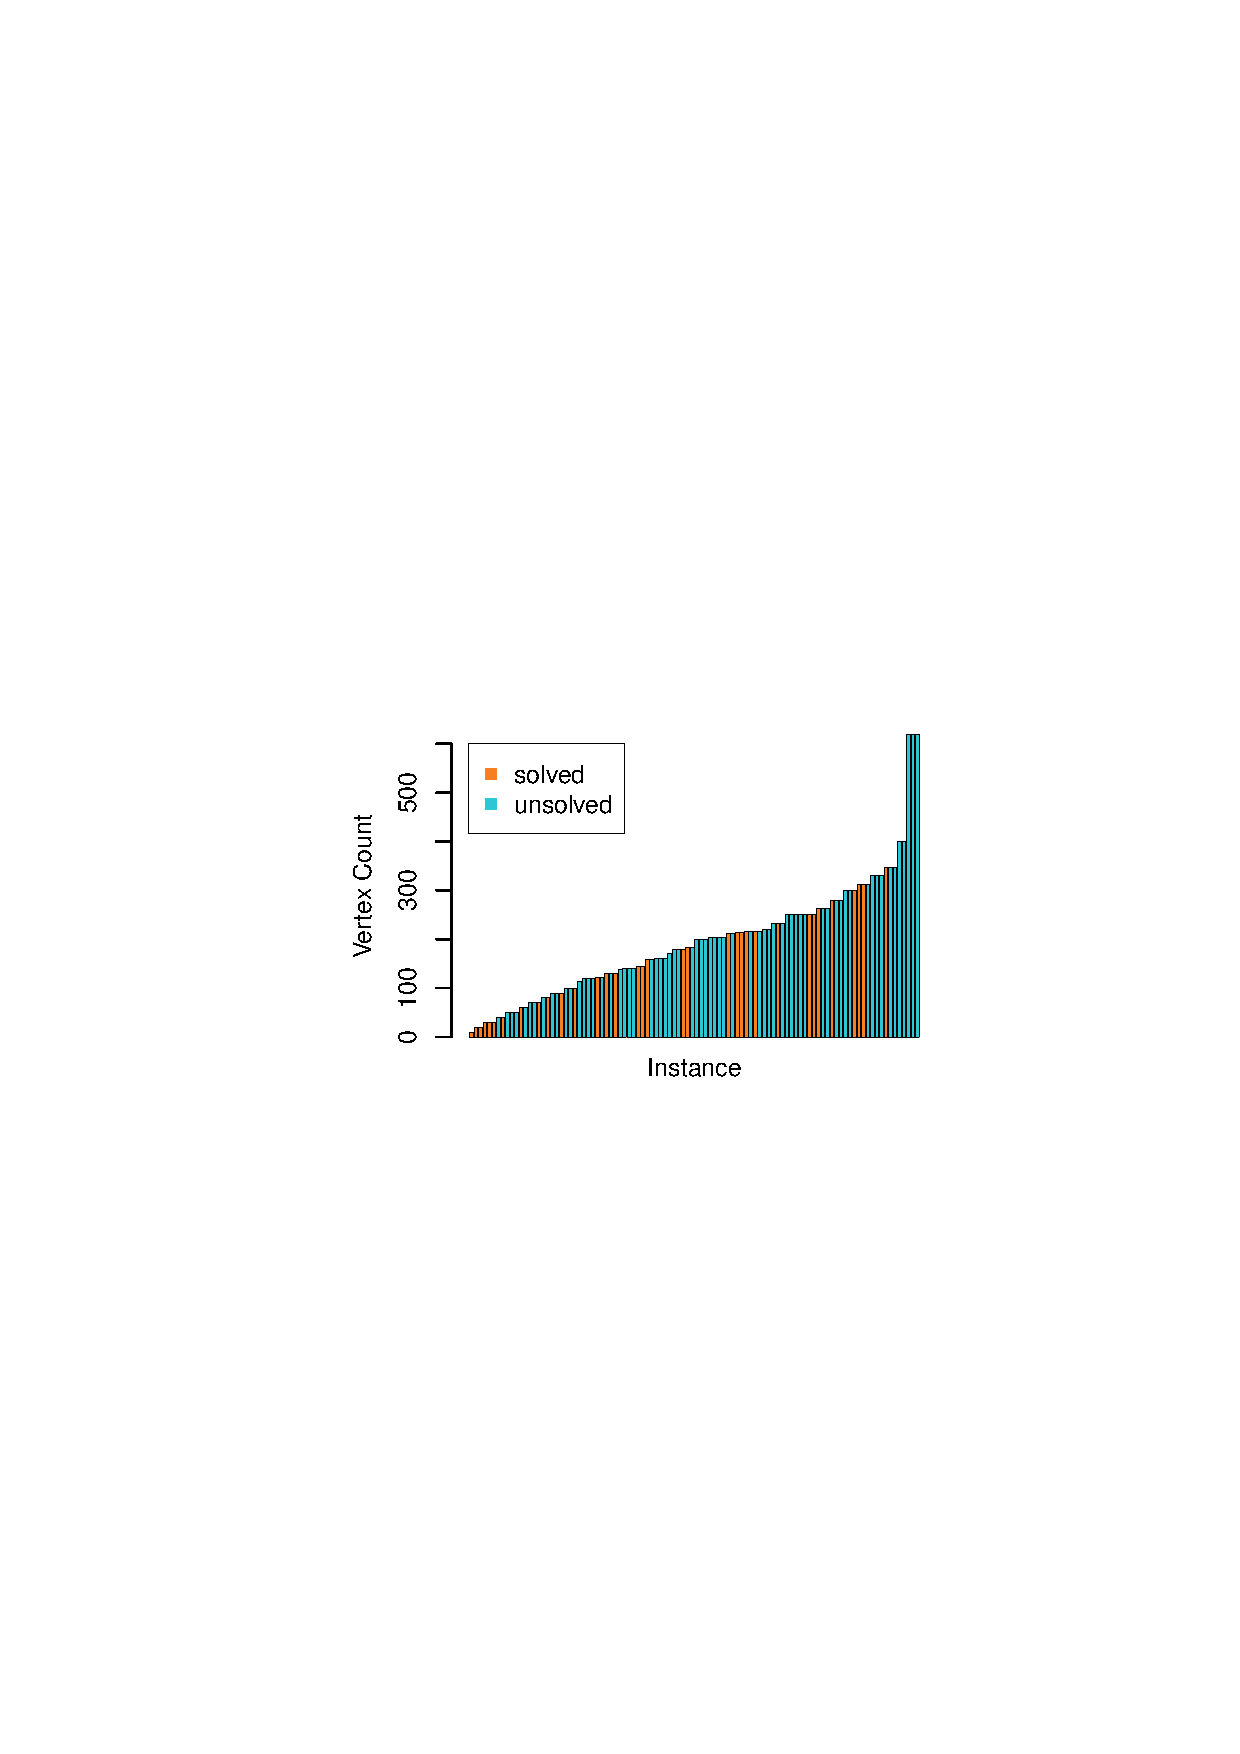
\includegraphics[width=1.0\linewidth]{instances}
		\subcaption{Instance Sizes}
	\end{subfigure}
	\begin{subfigure}{0.49\textwidth}
		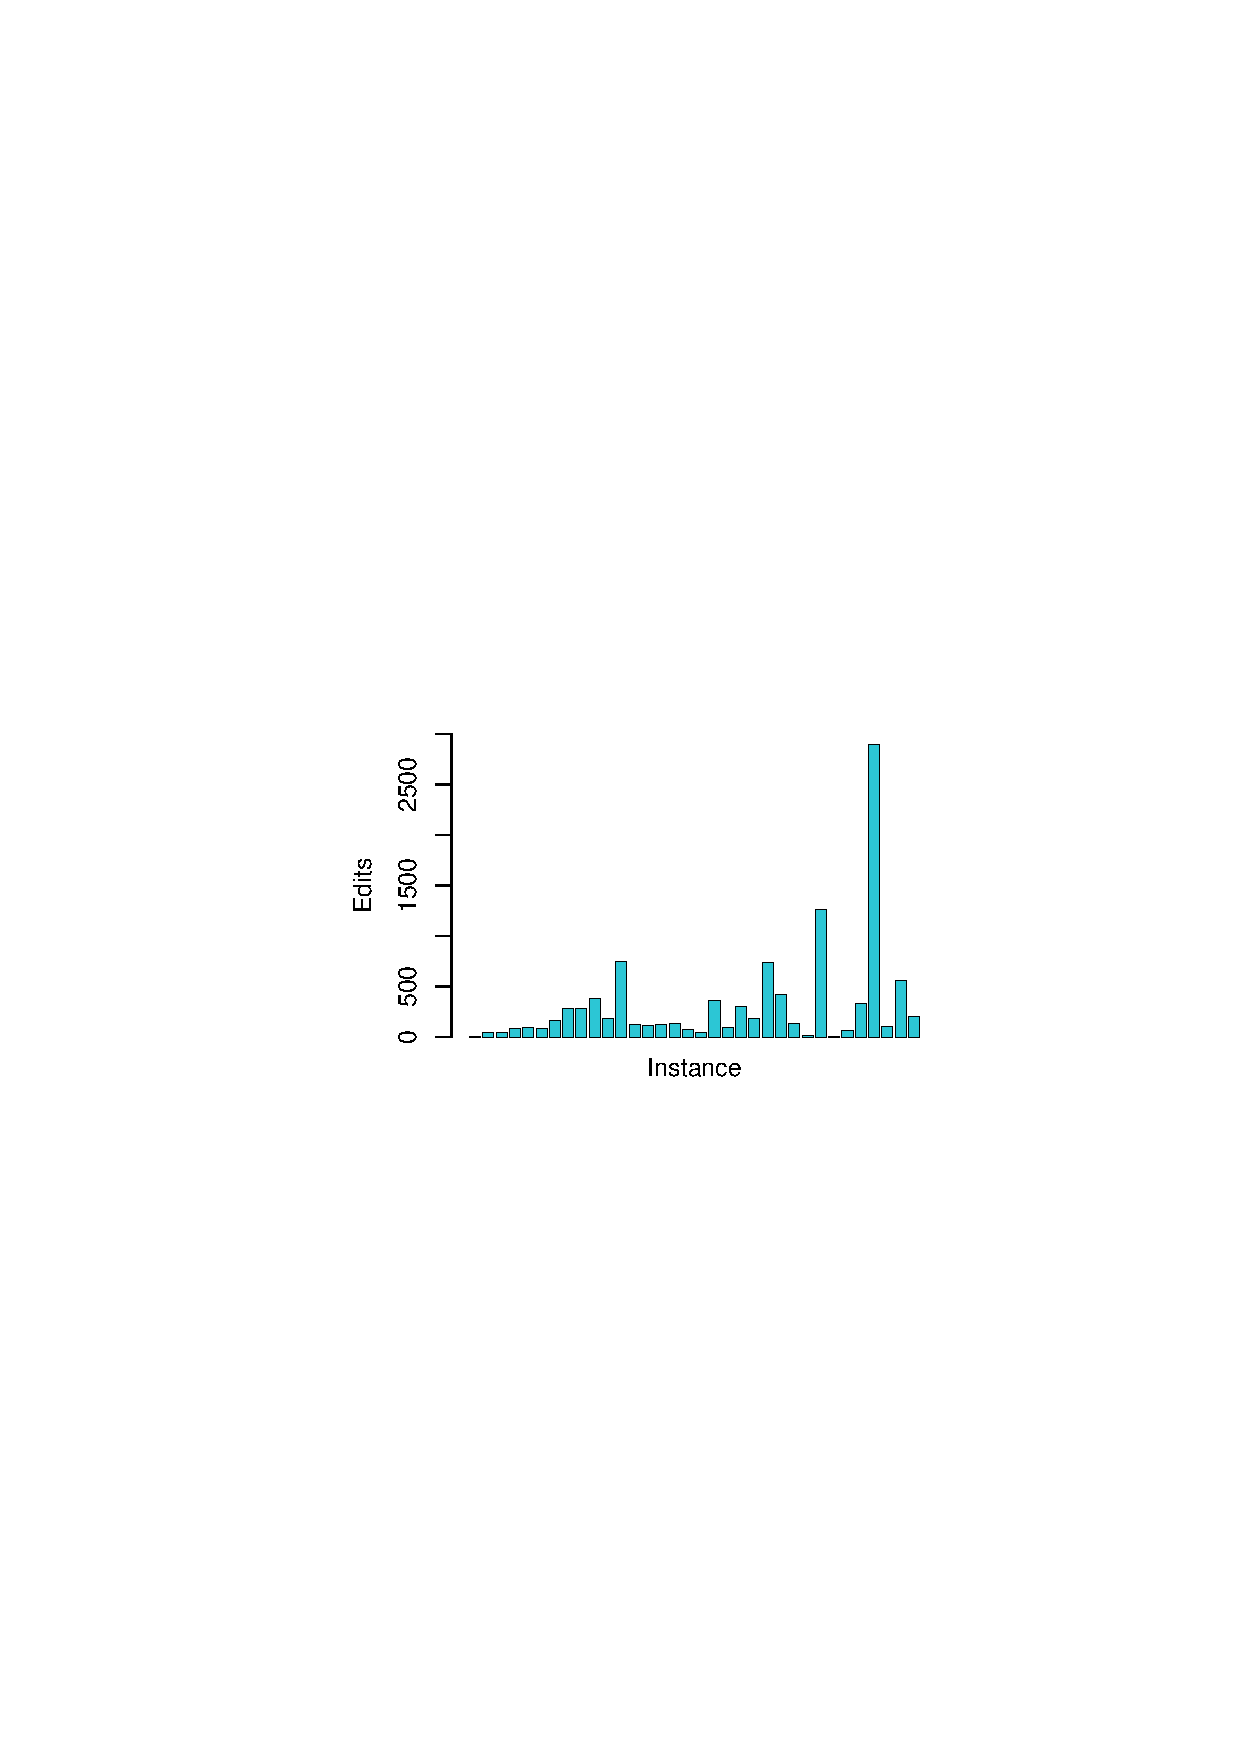
\includegraphics[width=1.0\linewidth]{solution_sizes}
		\subcaption{Solution Sizes}
	\end{subfigure}

	\caption{Public Problem Instances of the PACE Challenge}
	\label{fig:instances}
\end{figure}

\paragraph{Reduction effectiveness} We first present some results regarding the effectiveness of the
initial reduction steps. These are comparatively easy to measure as we can simply execute the
reduction on all instances and record the result. In Figure~\ref{fig:crit_clique eff} we give an
overview of how effective the critical clique reduction is for the test instances. Notably results
are very varied, with 35 instances not being reduced at all, one instance being almost solved
entirely (from 250 vertices in the input to 5 vertices), and other results at various places in
between. This is somewhat expected considering the critical clique approach ultimately doesn't
produce any edits, it only identifies and merges groups of vertices that are already cliques. Thus
the effectiveness is entirely subject to the structure of the input graph.

\begin{figure}[h]
	\begin{subfigure}{0.49\textwidth}
		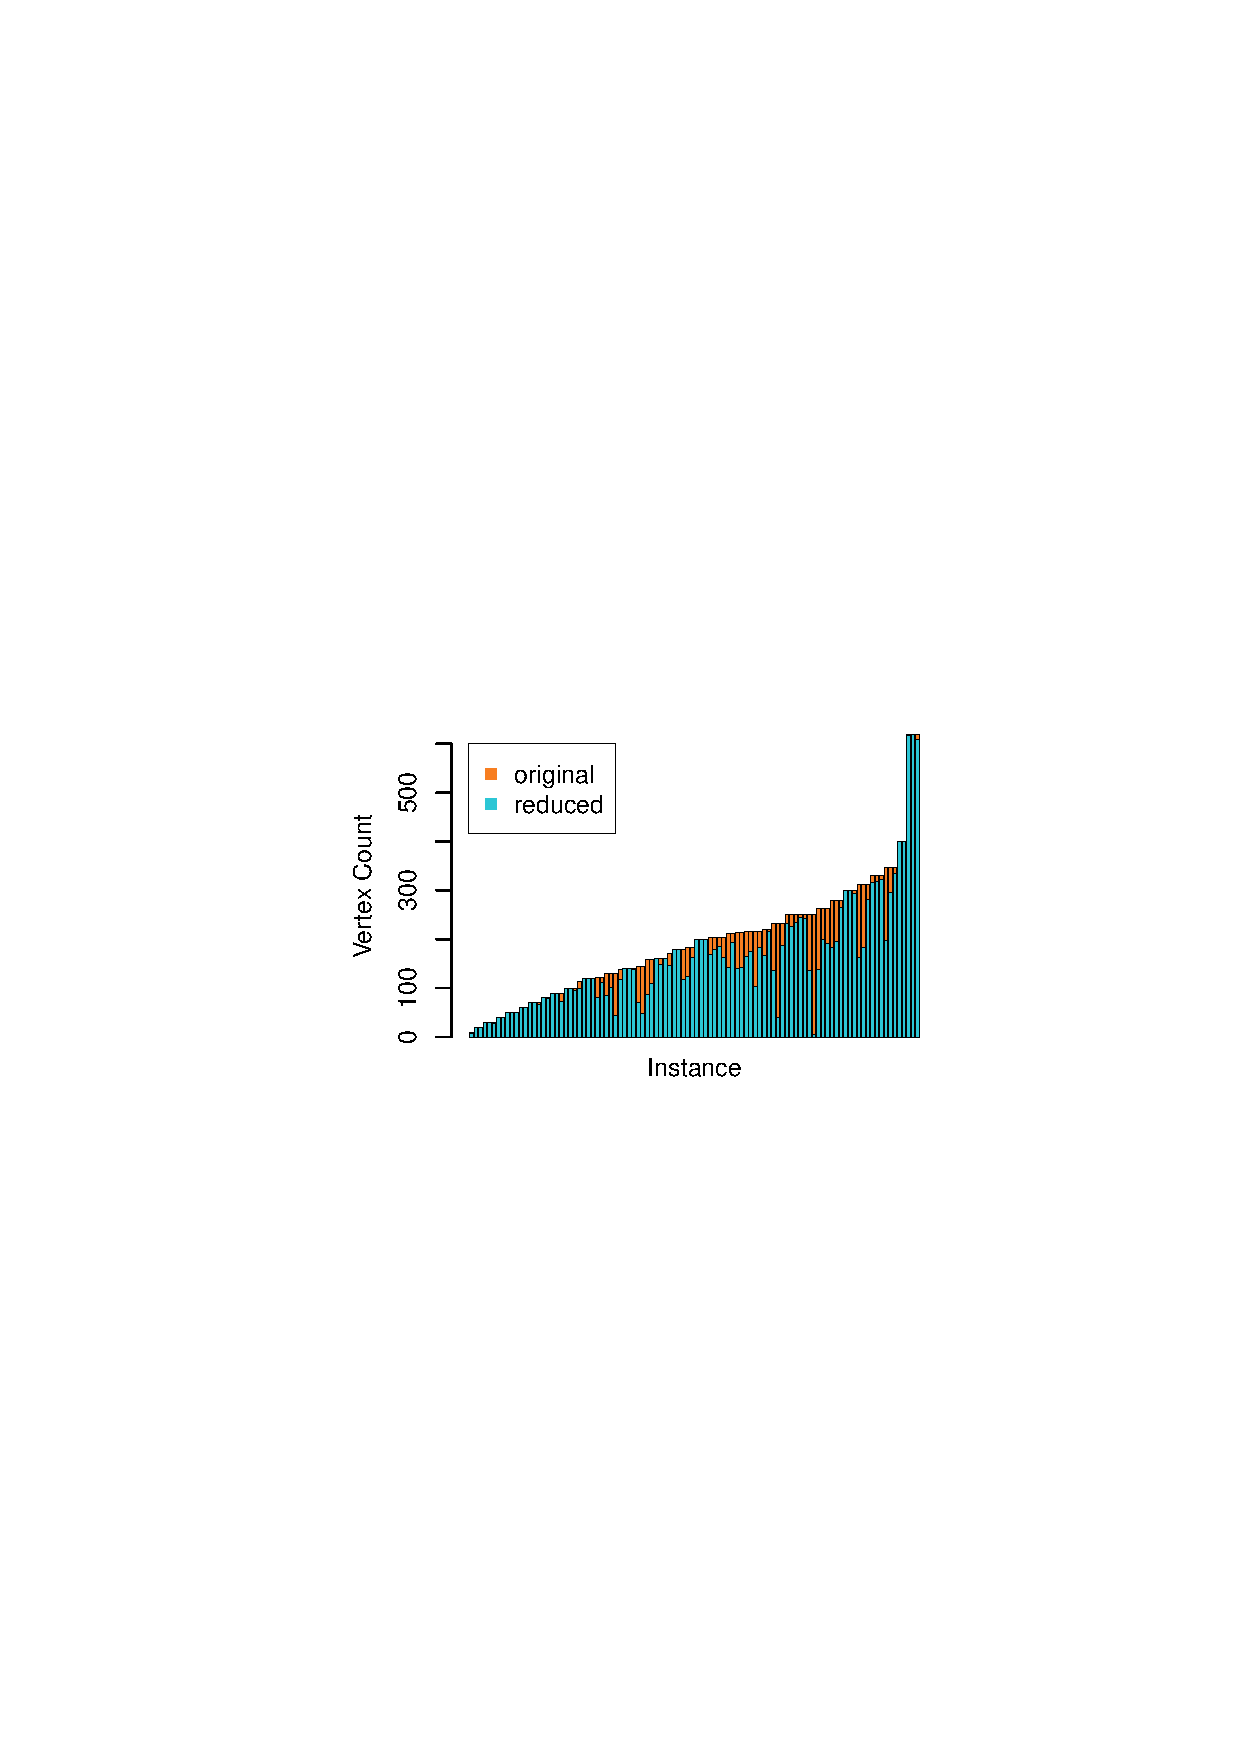
\includegraphics[width=1.0\linewidth]{crit_cliques_absolute}
	\end{subfigure}
	\begin{subfigure}{0.49\textwidth}
		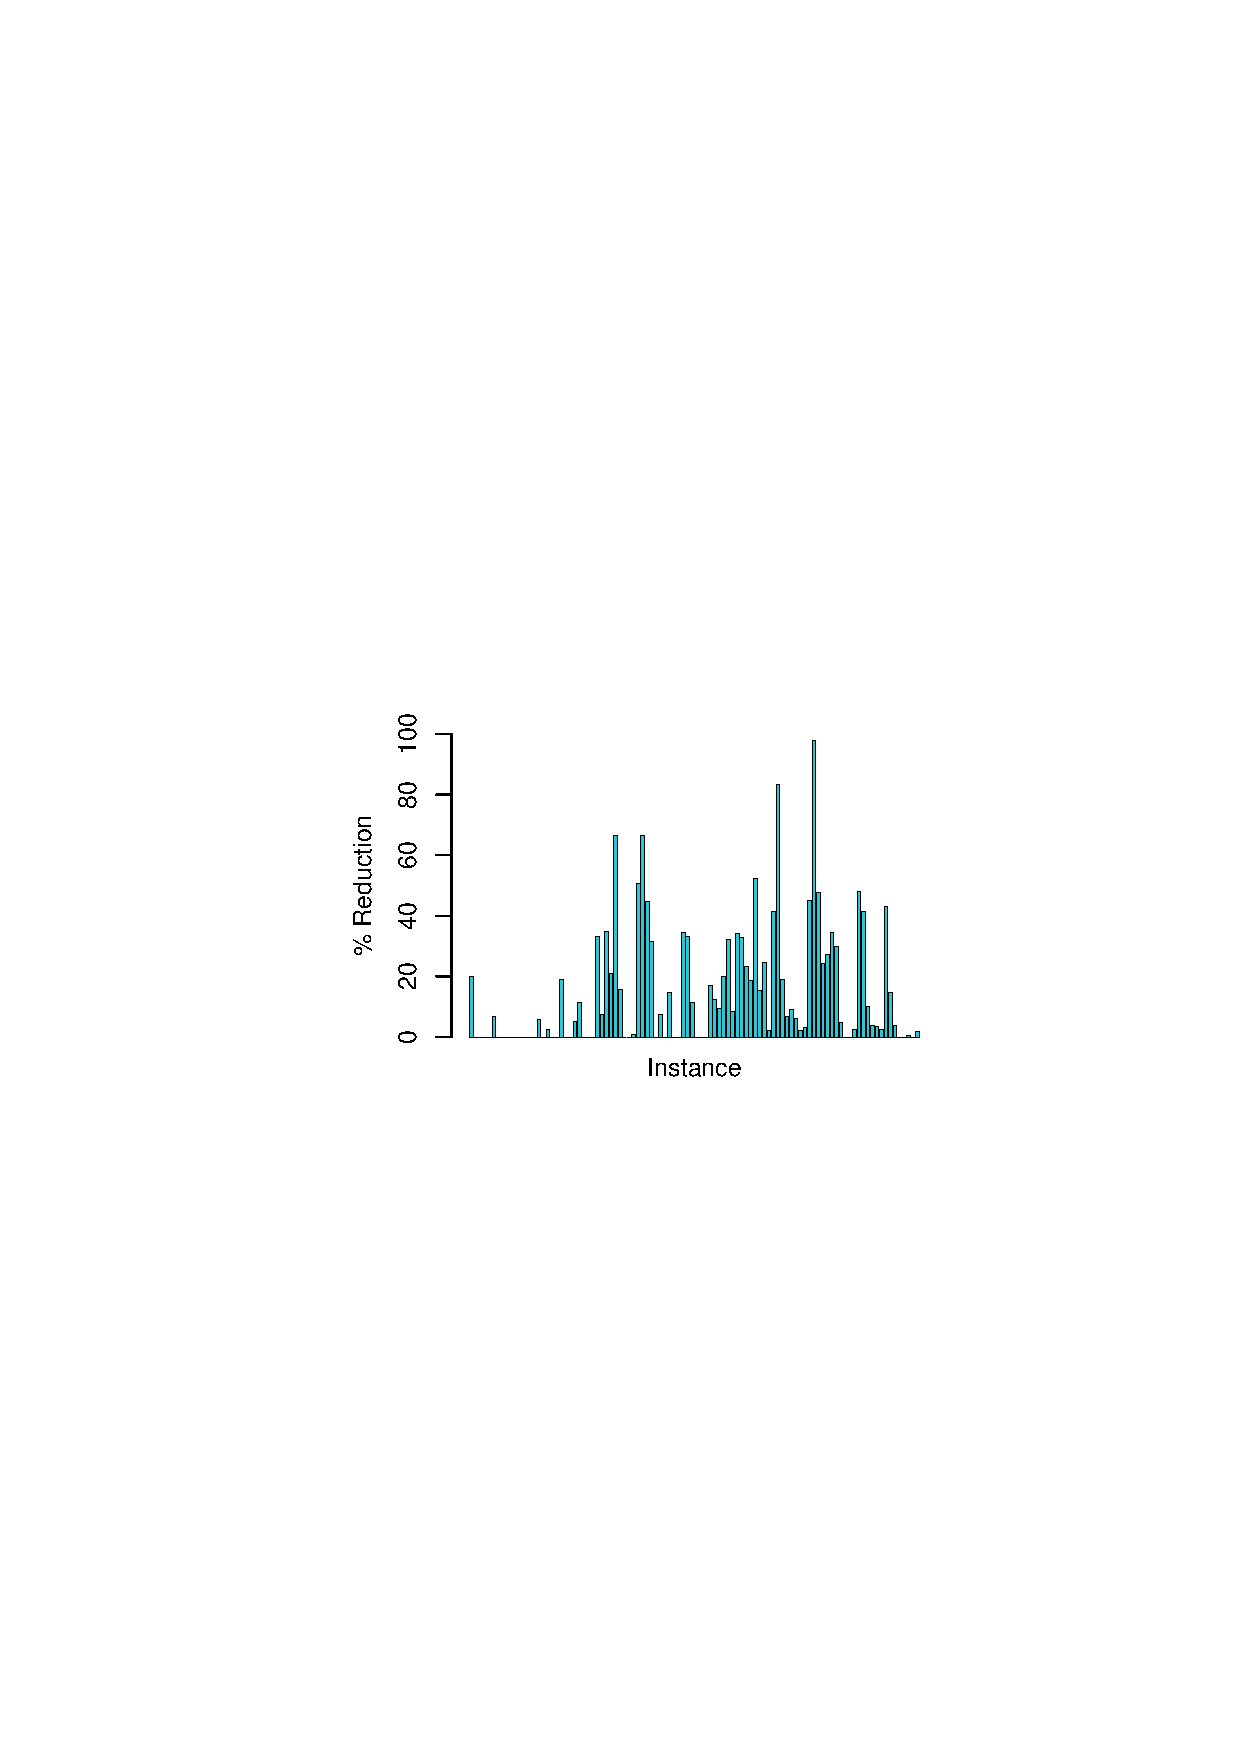
\includegraphics[width=1.0\linewidth]{crit_cliques_percent}
	\end{subfigure}
	\caption{Critical Clique Reduction Effectiveness}
	\label{fig:crit_clique eff}
\end{figure}

We present the same statistics for rules 1--5 applied together and for the complete initial
reduction in Figures~\ref{fig:rules1-5 eff} and~\ref{fig:initial eff}. Note that rule 1 forbids
edges instead of merging vertices, so it does not have a direct effect on these graphs (it may still
enable other reduction steps however). We observe that many of the larger peaks occur for the same
instance for both the critical clique reduction and rules 1--5. With Figure~\ref{fig:initial eff} we
can see that overall reduction is in fact most effective with all reductions enabled, as expected.
Considering the negligible runtime of the reductions on graphs of the size used in the challenge, it
is definitely reasonable to always run the full set.

\begin{figure}[h]
	\begin{subfigure}{0.49\textwidth}
		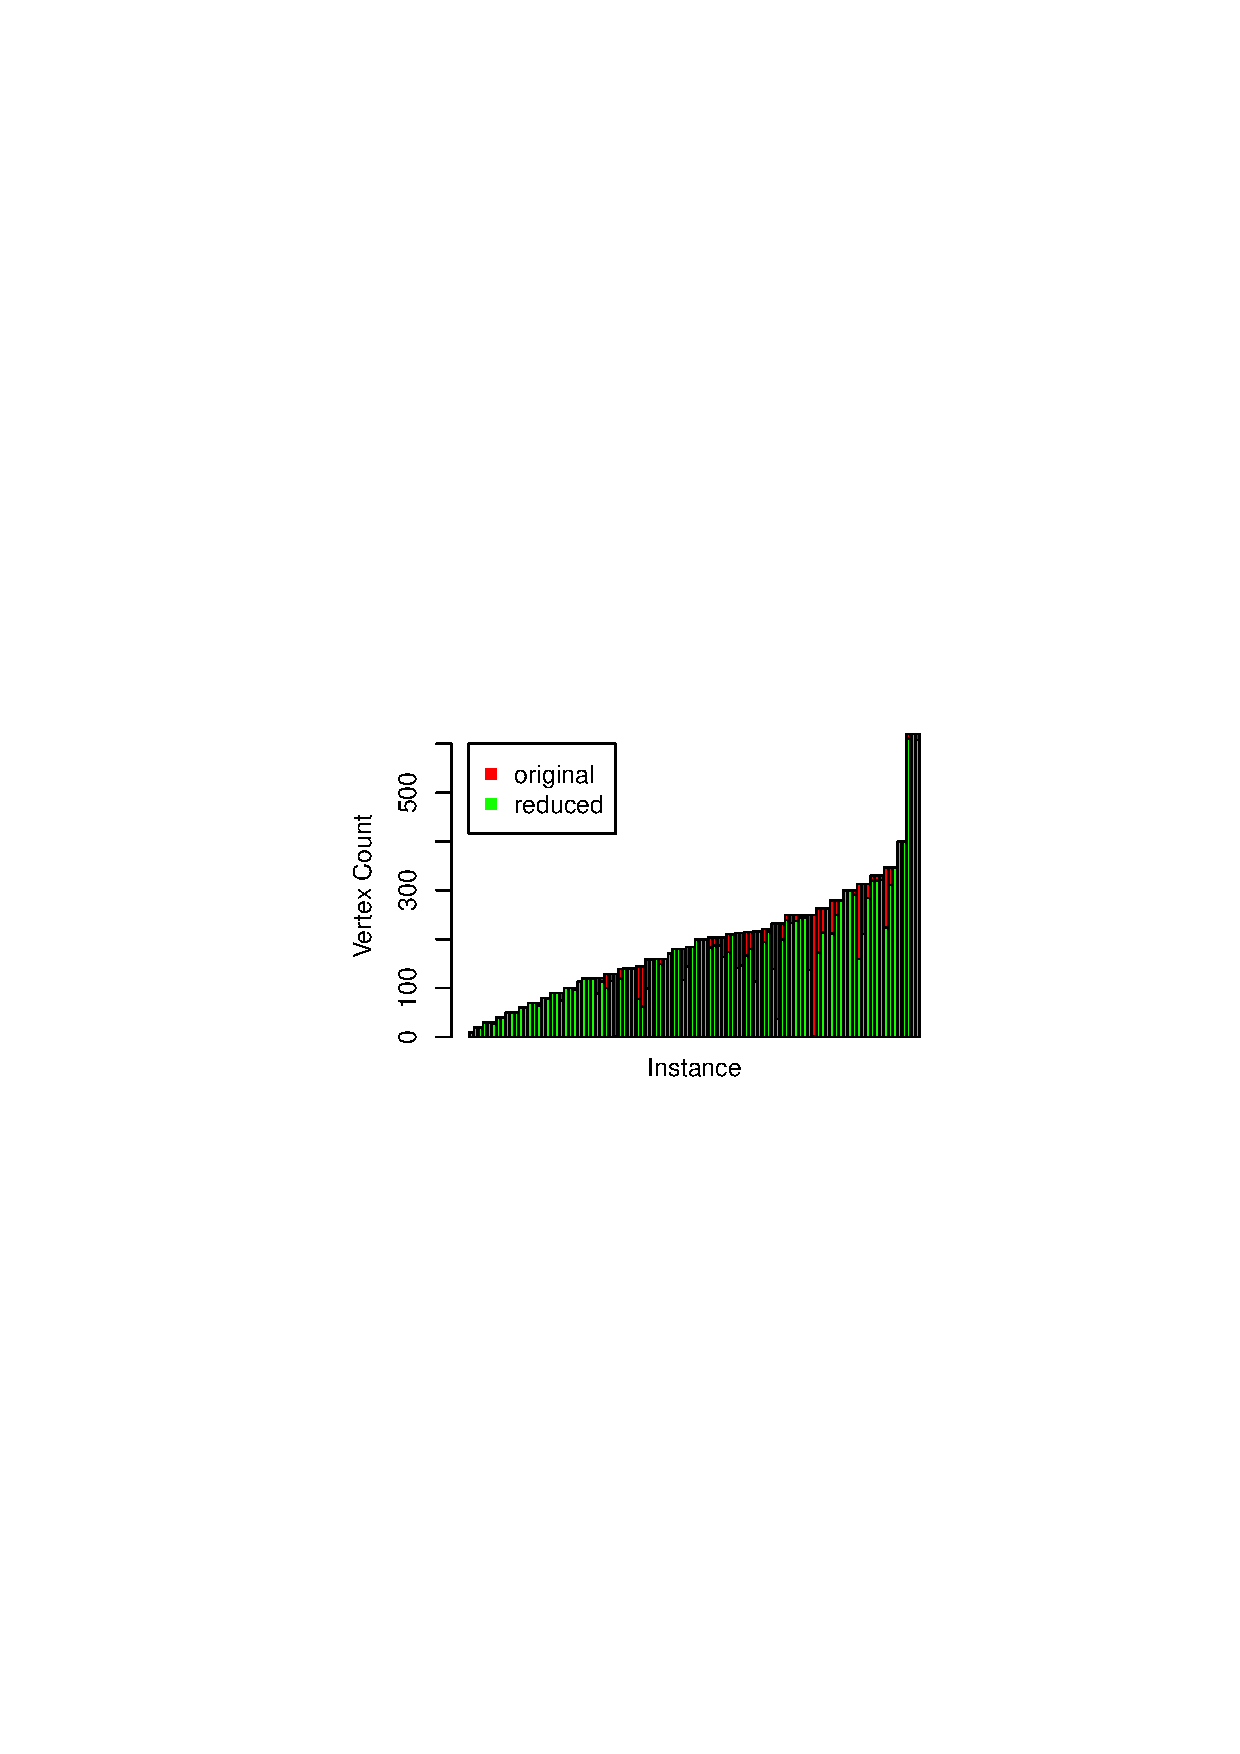
\includegraphics[width=1.0\linewidth]{rules1-5_absolute}
	\end{subfigure}
	\begin{subfigure}{0.49\textwidth}
		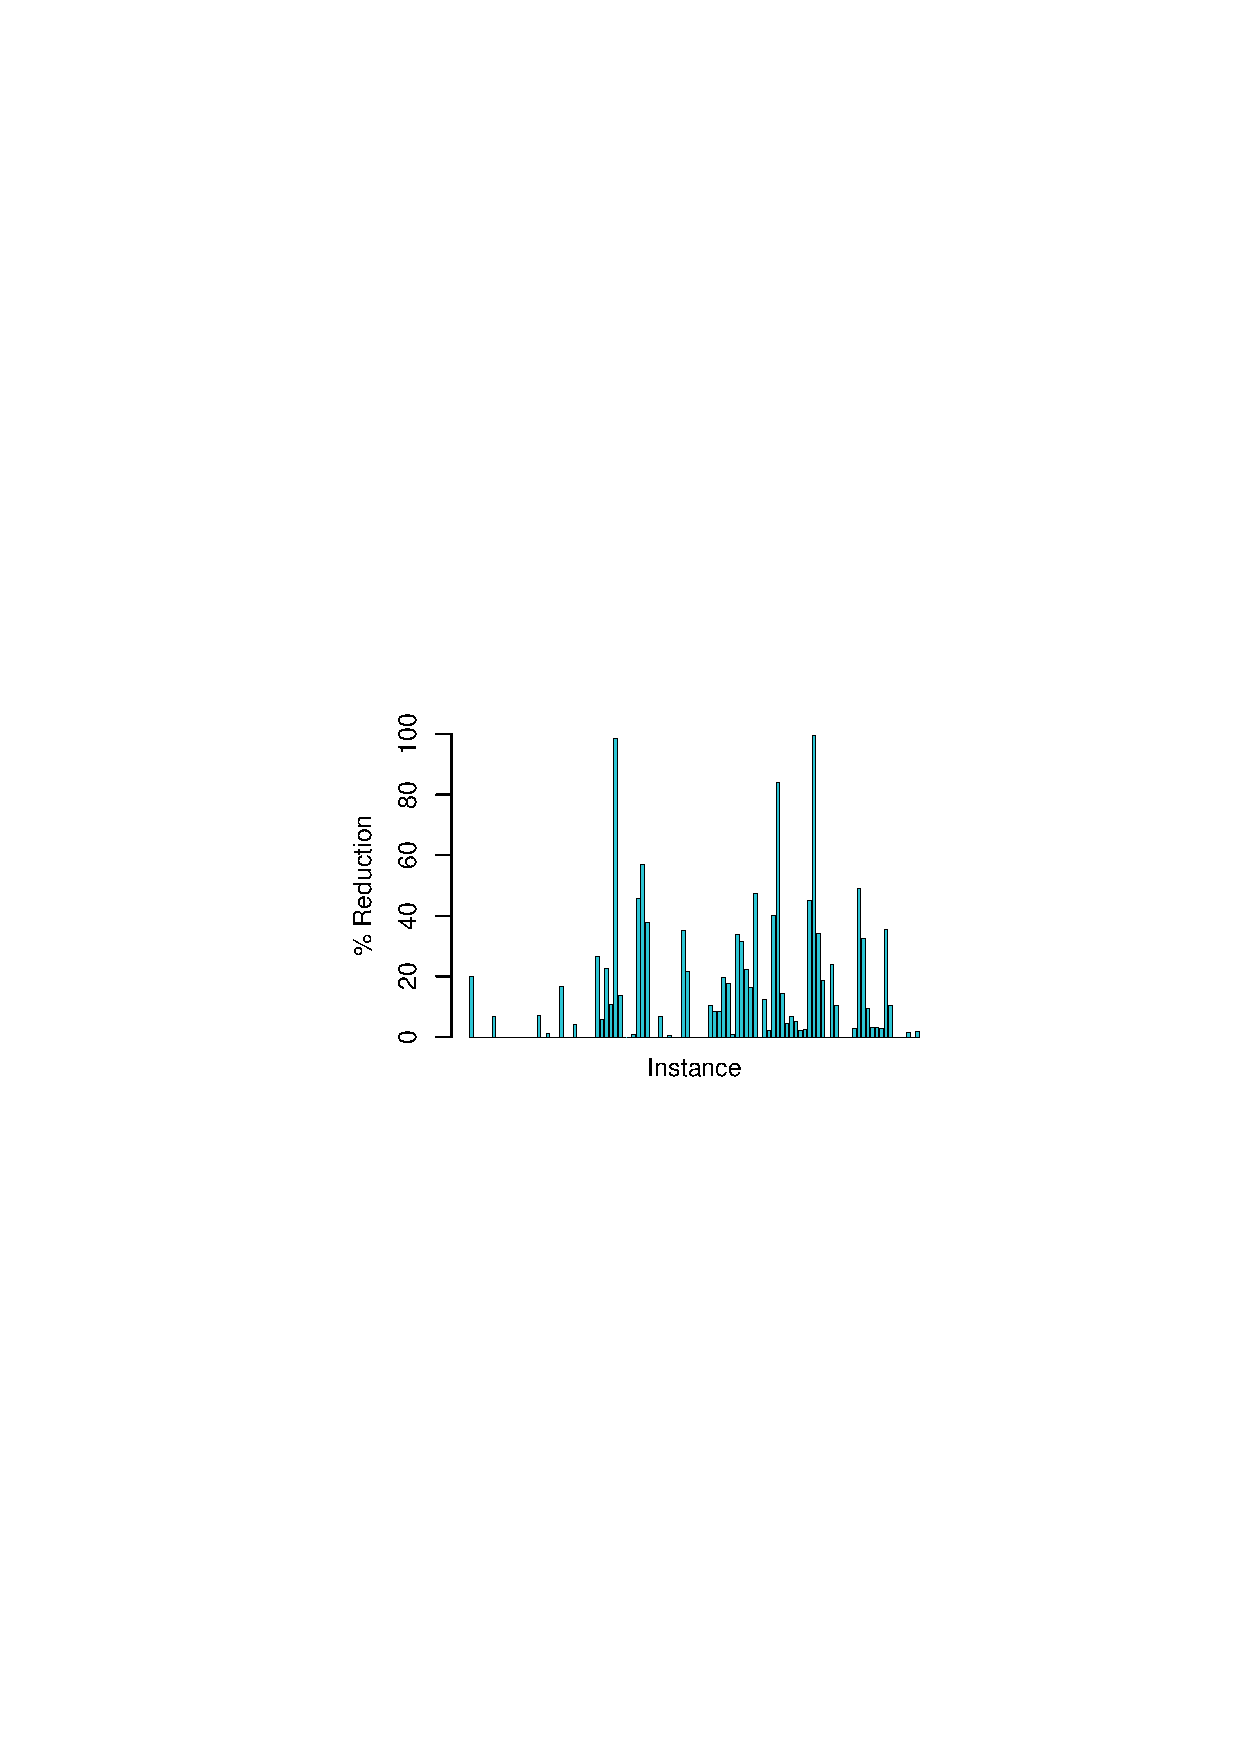
\includegraphics[width=1.0\linewidth]{rules1-5_percent}
	\end{subfigure}
	\caption{Rules 1--5 Effectiveness}
	\label{fig:rules1-5 eff}
\end{figure}

\begin{figure}[h]
	\begin{subfigure}{0.49\textwidth}
		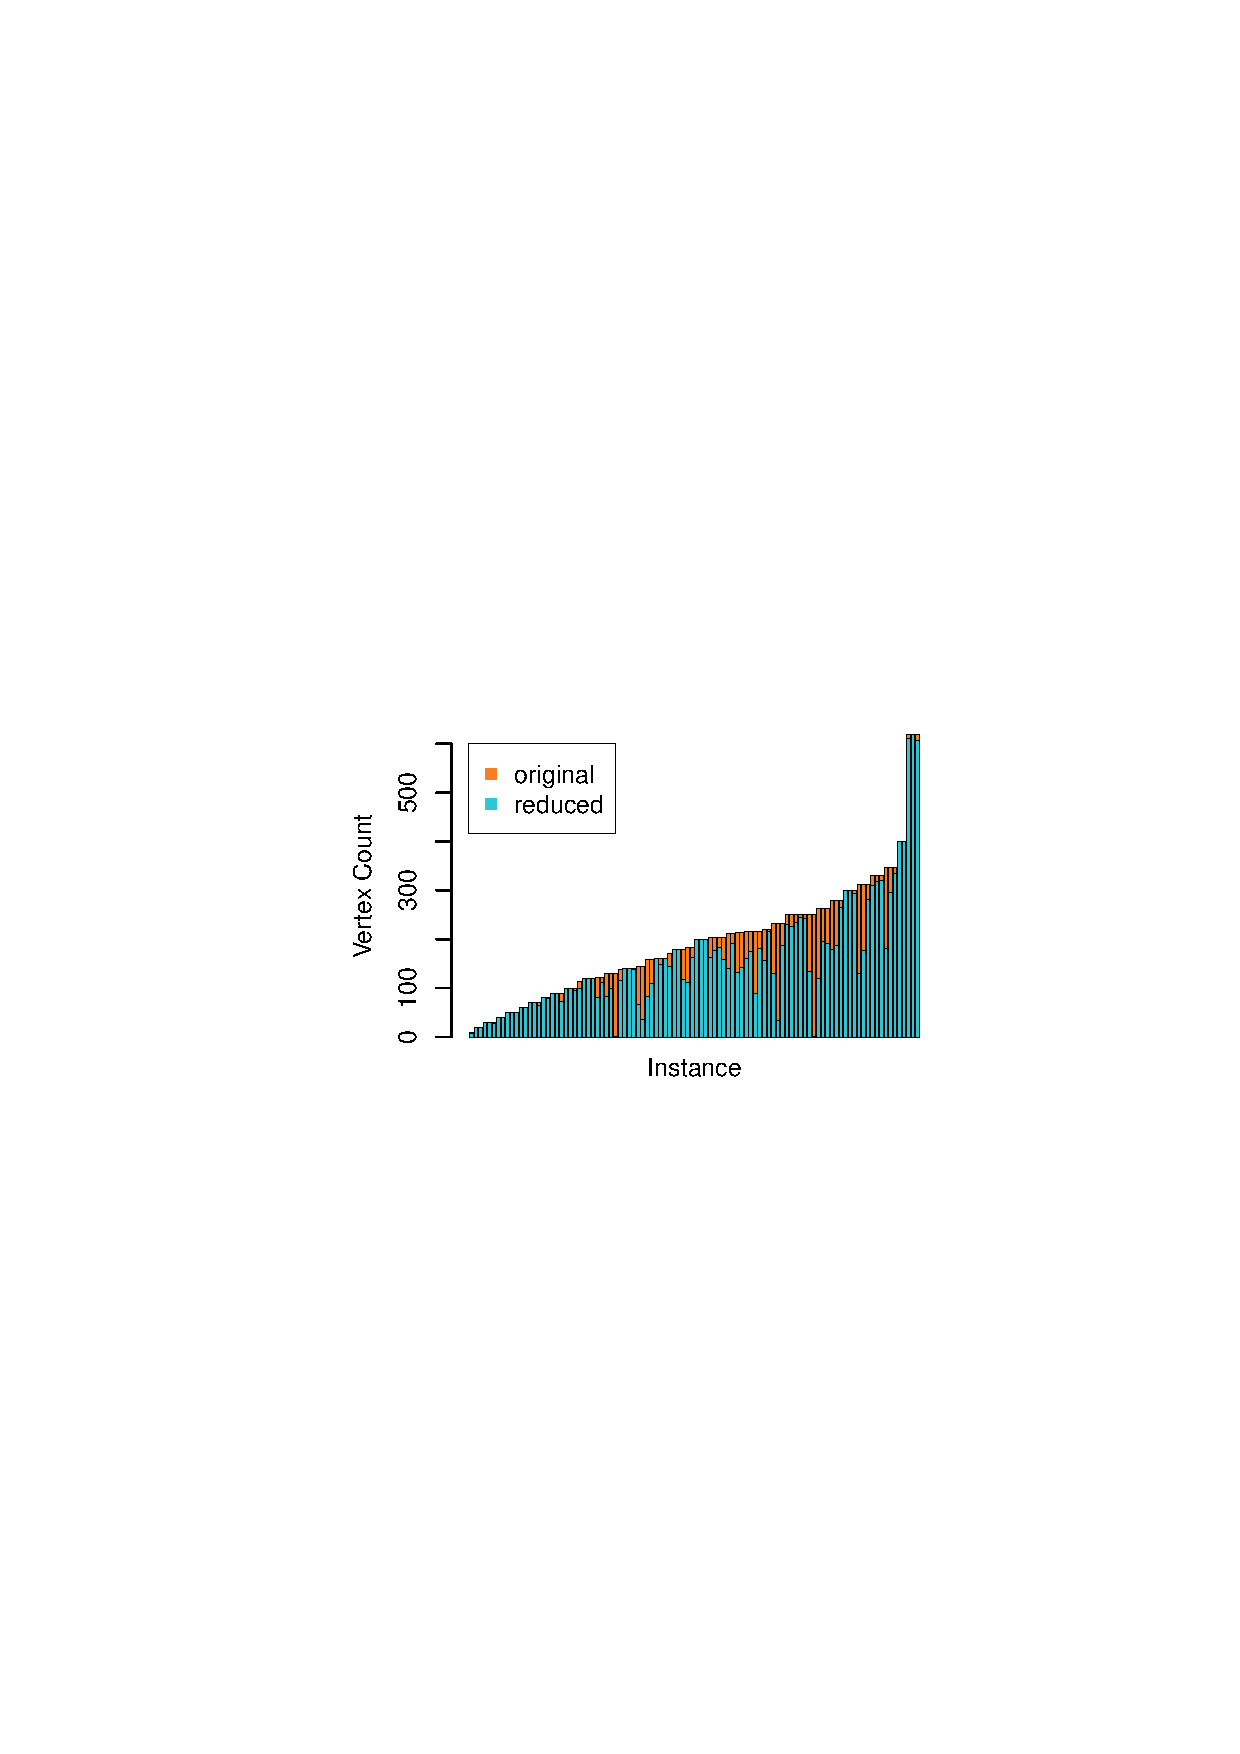
\includegraphics[width=1.0\linewidth]{full_initial_absolute}
	\end{subfigure}
	\begin{subfigure}{0.49\textwidth}
		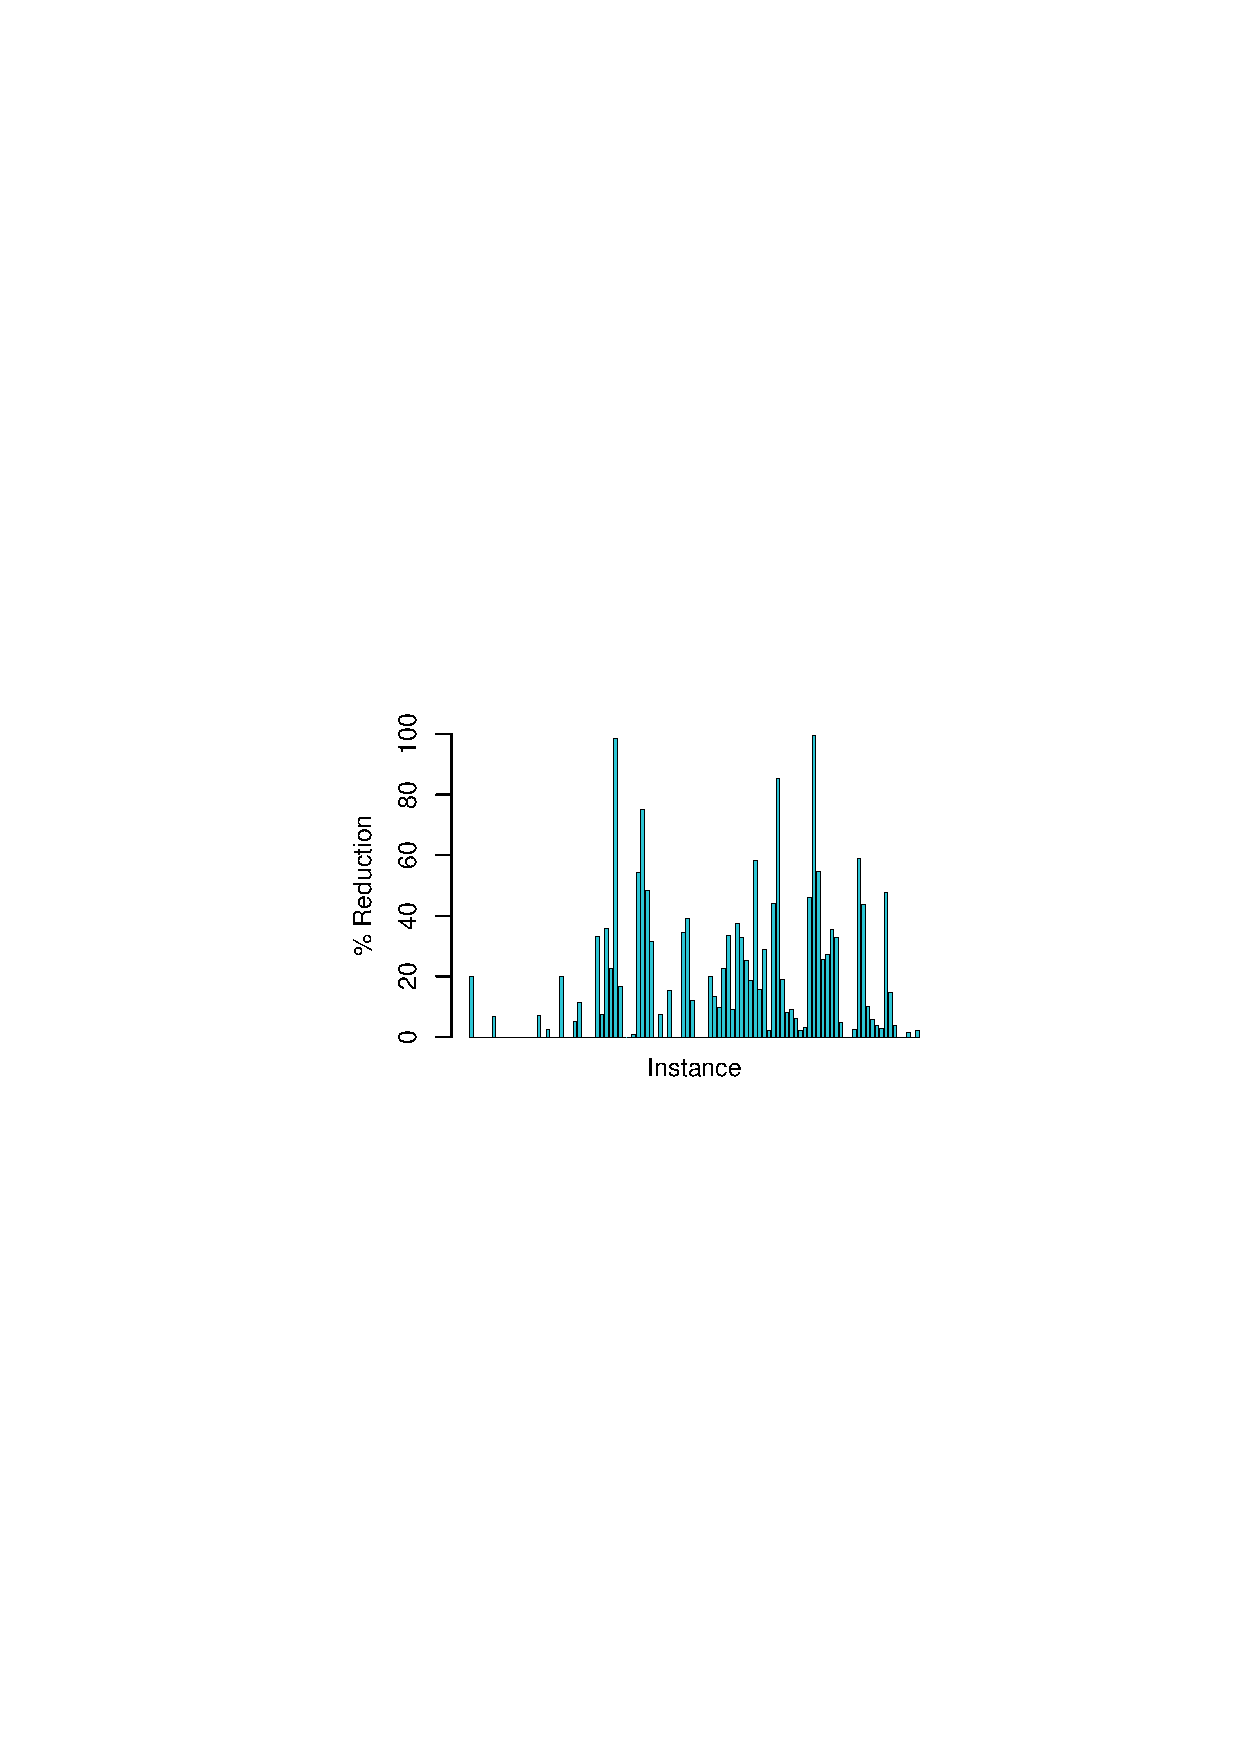
\includegraphics[width=1.0\linewidth]{full_initial_percent}
	\end{subfigure}
	\caption{Full Initial Reduction Effectiveness}
	\label{fig:initial eff}
\end{figure}

An additional factor to consider is that while the effectiveness of the critical clique reduction is
fully captured in the size of the reduced graphs, the same is not true for the other reductions.
While most of them (with the exception of rule 1) also perform merging of vertices as their only
operation on the graph, this can also result in various additional edits, hopefully making the
complete solution easier to find. For an impression of how effective the reductions are in this
regard, in Figure~\ref{fig:edits from reduction} we show what percentage of the amount of edits in
an optimal solution is found by the reductions (for the 34 instances we have solved so far).
Comparing the full set of reductions with only using rules 1--5, we can see that while the critical
clique reduction does not produce any edits on its own, the simplified graph it produces is easier
to reduce by the other rules.

\begin{figure}[h]
	\begin{subfigure}{0.49\textwidth}
		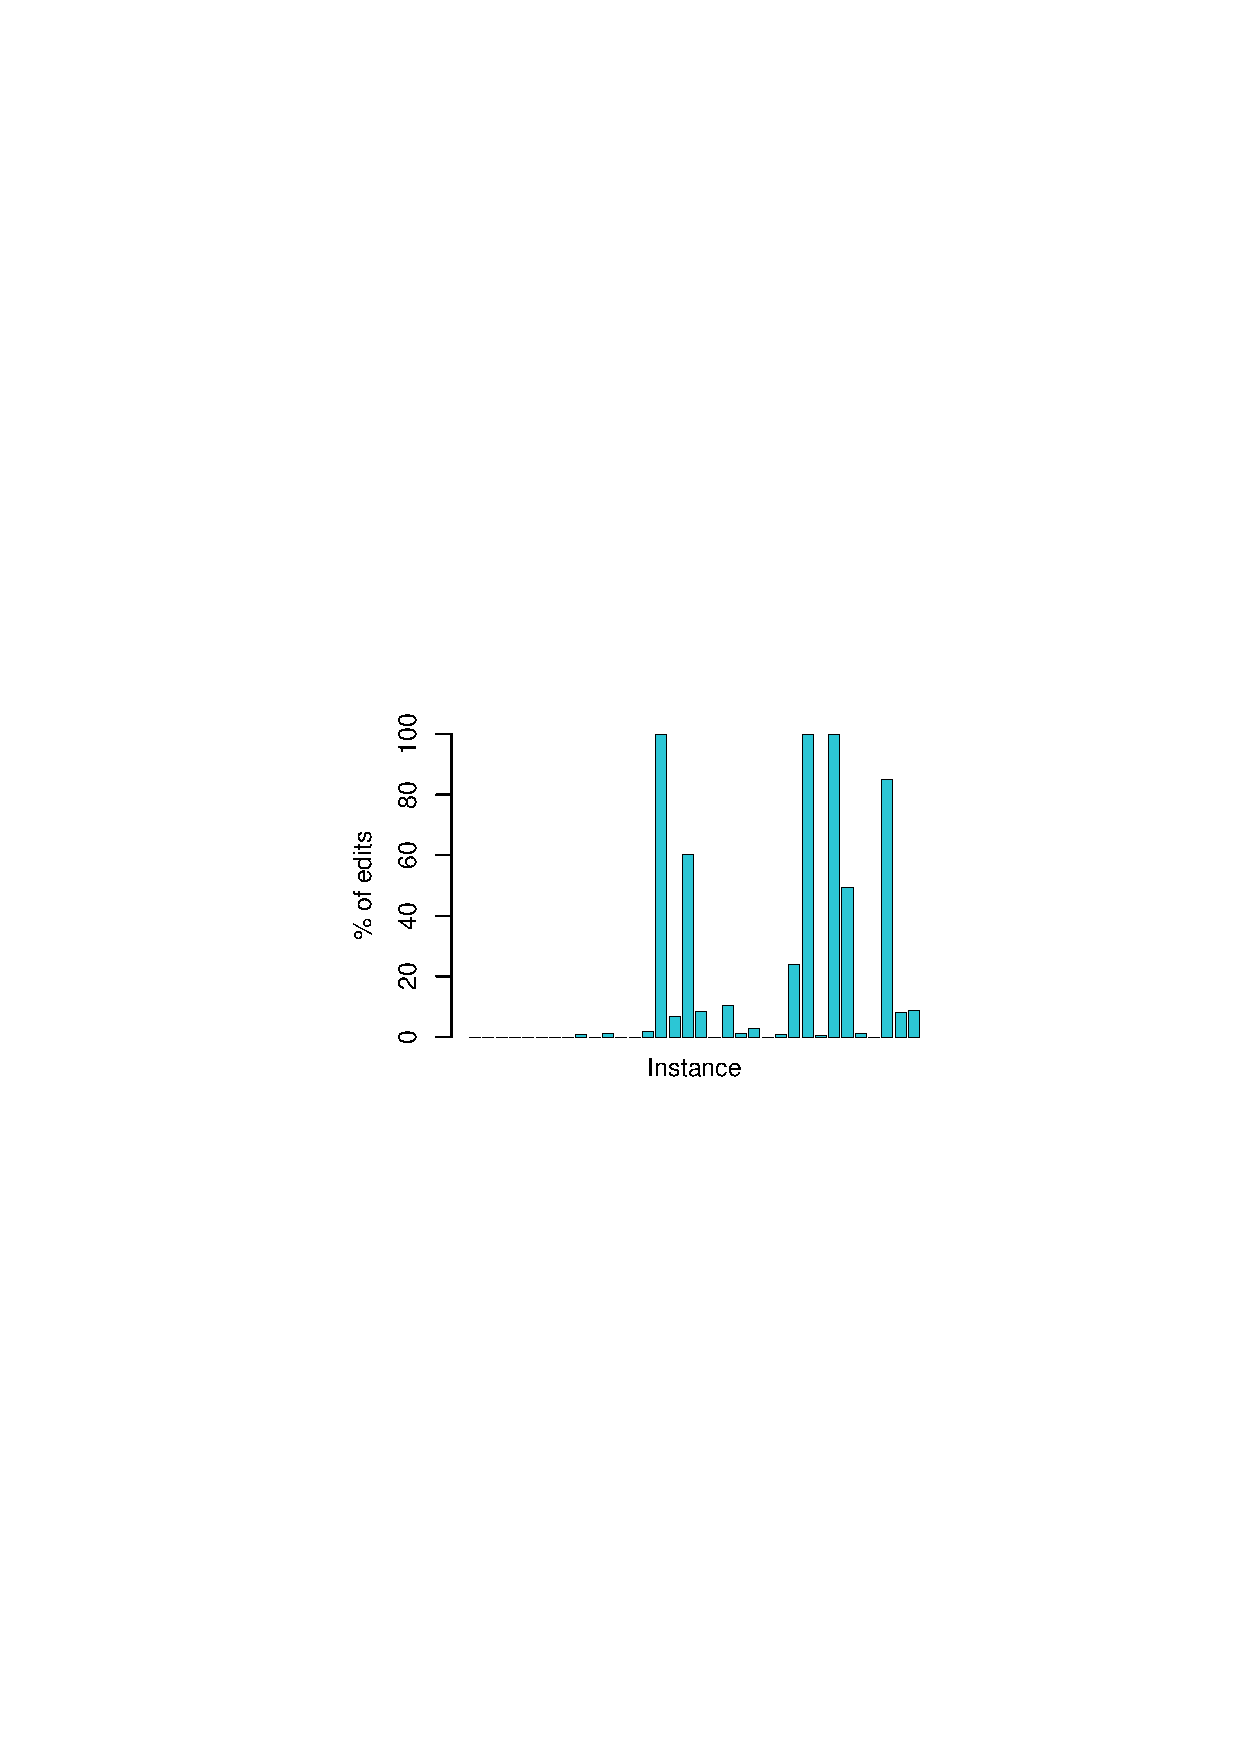
\includegraphics[width=1.0\linewidth]{percent_edits_full}
		\subcaption{Full Initial Reduction}
	\end{subfigure}
	\begin{subfigure}{0.49\textwidth}
		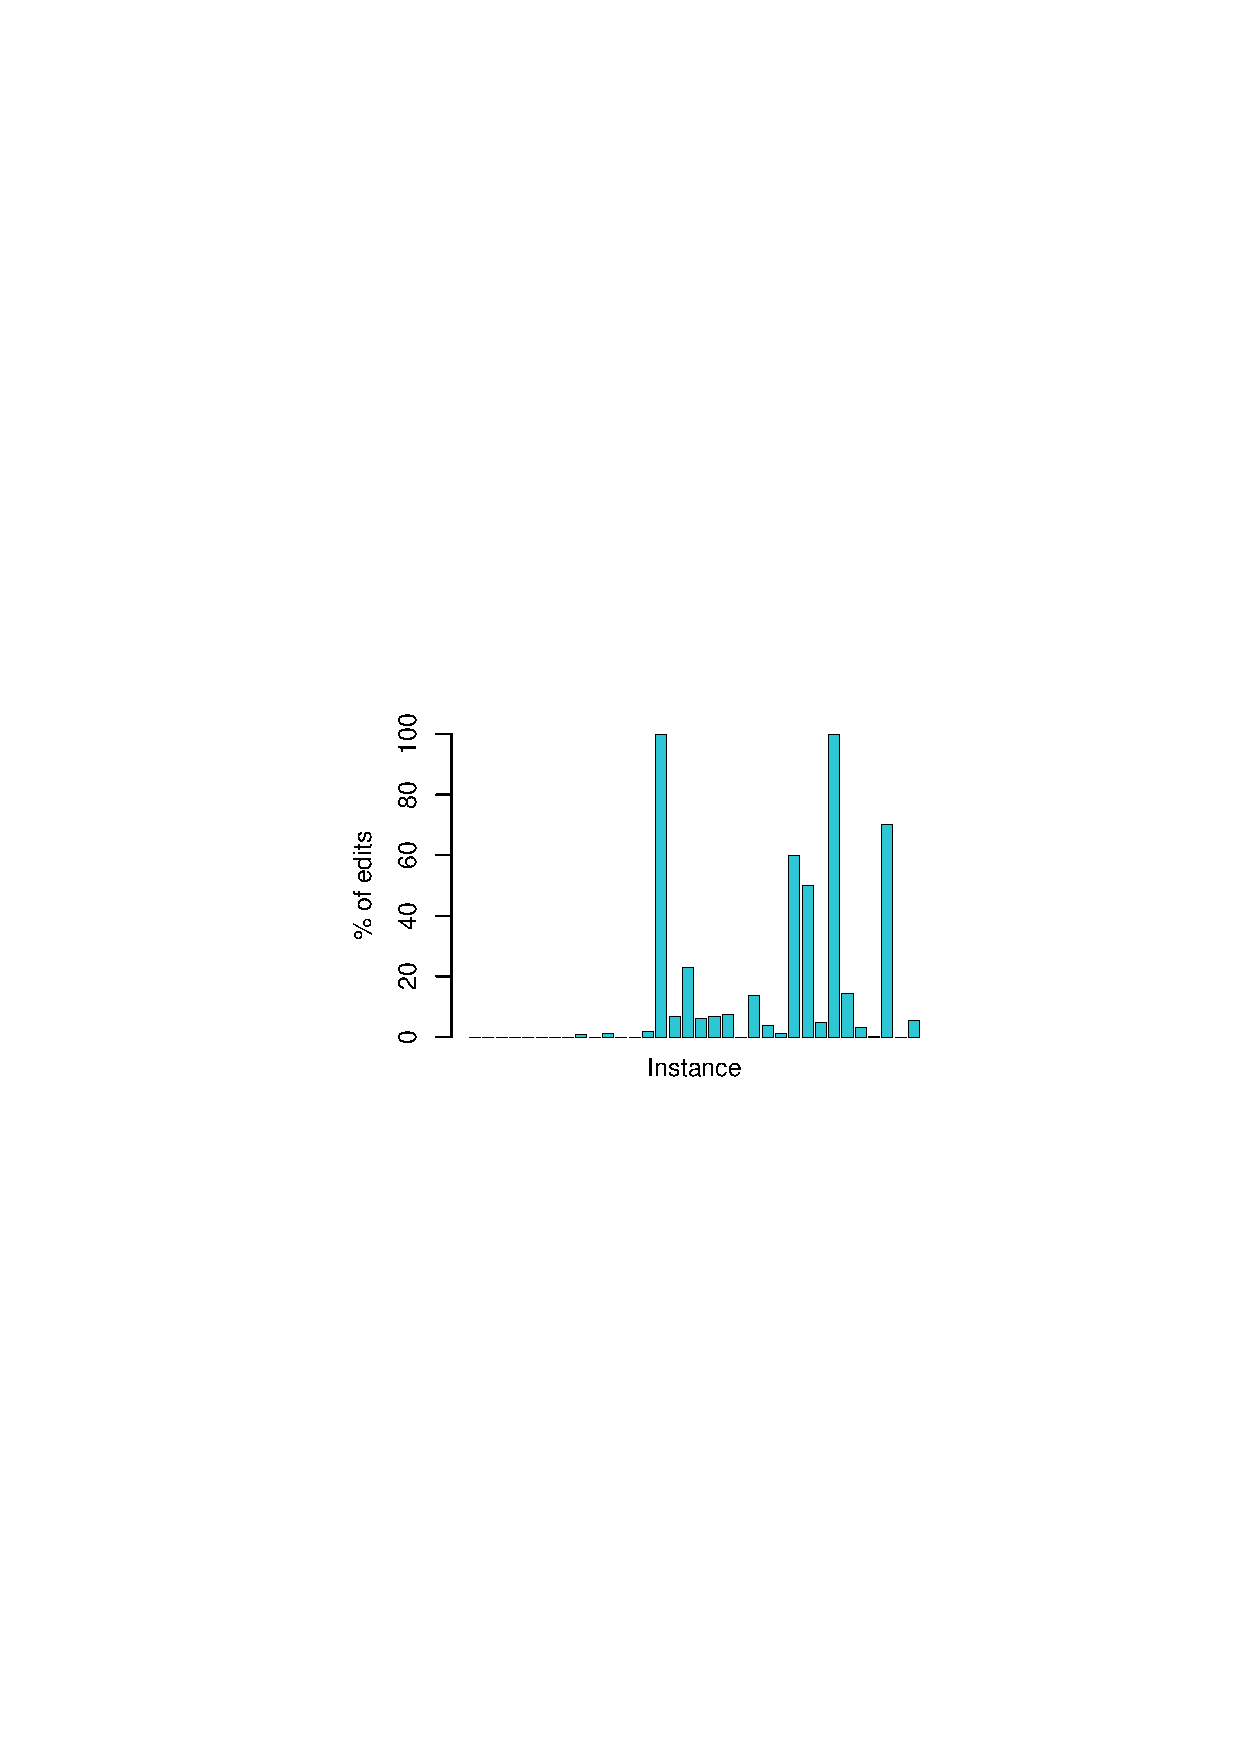
\includegraphics[width=1.0\linewidth]{percent_edits_rules1-5}
		\subcaption{Only rules 1--5}
	\end{subfigure}
	\caption{\% of edits of an optimal solution found by initial reduction steps}
	\label{fig:edits from reduction}
\end{figure}

As described in section~\ref{sec:reduction}, we apply all reduction rules except for the critical
clique reduction at points in the search tree too. It is somewhat harder to accurately measure the
effectiveness of this, but we can at least get an impression of which rules are how effective. To
this end, we measured how much ``reduction in $k$'' each reduction, as well as the branching
decisions themselves, resulted in over the course of solving a whole instance. For every branch that
is explored, whenever $k$ is reduced due to some operation, we attribute this reduction to one the
mentioned causes. If we exit early from some brunch, due to our lower bounds, the remaining
parameter is attributed to ``early exit''. Note that this measurement is hardly perfect. For example
exiting early with parameter $k$ attributes $k$ to early exit, but if we had explored the tree
further down this path, there would have been more reduction observed in total, so the effect of
early exiting is in some way underrepresented. We have also implemented a much more accurate and
detailed form of collecting statistics around the effectiveness of reductions, but it is
unfortunately much harder to analyze, and, more importantly, incurs so much overhead in its current
implementation that it is impractical to use for anything but the smallest and easiest-to-solve
instances.

With that in mind, Figure~\ref{fig:interleaved_effectiveness} summarizes the results of the
described estimation. Clearly with our current settings, the induced cost reduction provides a very
large portion of our performance. To some extent this likely just reflects our current choice of
parameters for the solver: We execute rules 1--5 only once every 200 nodes along a path in the tree,
while we execute the induced cost reductions at every single node. Even on the nodes where we
execute the full reduction, we first execute the induced cost reduction followed by rules 1--5. Our
testing so far has shown these settings to be effective in achieving good runtime on our test
instance, but it is possible a different combination could lead to still improved performance,
perhaps resulting in a more balanced mix in the effectiveness of the reductions. Even with that in
mind, these results do match our experience developing the solver: Implementing the induced cost
reduction was one of the biggest single improvements we have observed, even though rules 1--5 were
implemented first (and executed much more frequently before then.)

\begin{figure}[h]
	\centering
	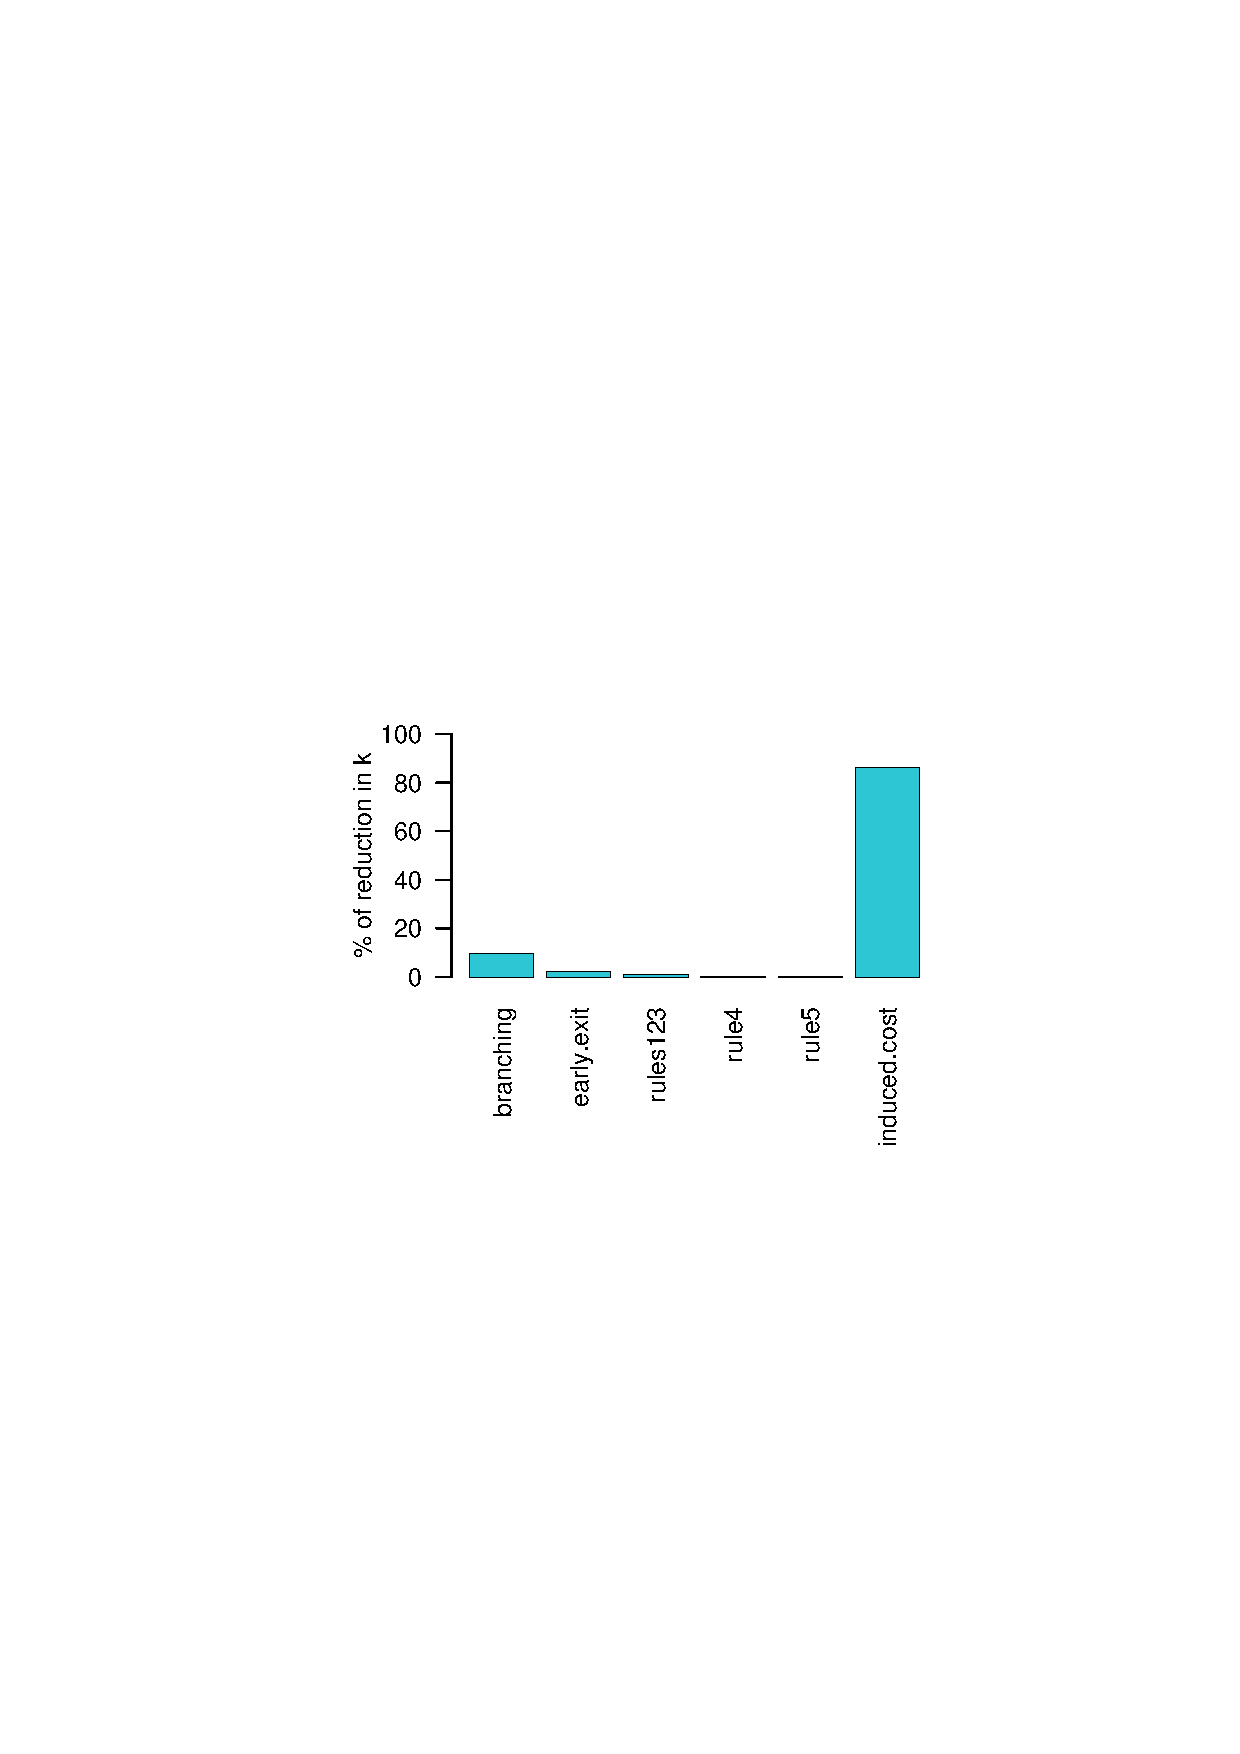
\includegraphics[scale=0.8]{interleaved_effectiveness}
	\caption{\% of total reduction in $k$ by source, averaged over all solved instances}
	\label{fig:interleaved_effectiveness}
\end{figure}

\todo if there is time left, do some more testing for this perhaps

\todo would also be nice to do another run with more balanced settings just to compare the
effectiveness results

\todo a SLURM run is ongoing to get this graph but with stats for *all* solvable instances, update
this when it's done

\todo

\begin{itemize}
	\item Maybe more on parameter-tuning (reduction intervals) (any graphs or something? have to see
		if there's enough time to run good tests for this)
	\item What techniques provided what kind of benefit as they were introduced, what did we try
		that wasn't worth it?
\end{itemize}

\chapter{Outlook \& Conclusion}

We plan to continue work on the solver until the submission deadline for the PACE challenge. There
are still many potential options for improvement: Parameters for tweaking the behavior of the
solver can be optimized. There is likely room for optimization in the existing implementation. More
reduction rules can be implemented and tested, as well as the strategy for applying the current ones
improved. We are also planning to try the more advanced branching strategies by Böcker et
al.~\cite{GoldenRatio}

An additional avenue potentially worth investigating is supporting multithreading in the solver, or
potentially allowing splitting computation over multiple instances of the solver to support usage on
a cluster of compute nodes. In the context of the PACE challenge, the solver can only make use of
one core, so we have not pursued this so far. For practical applications it could however provide a
significant benefit. There are several approaches that would allow splitting up the work to be
performed in parallel relatively straightforwardly. We also have the additional advantage of our
solver being written in Rust, which can guarantee thread-safety statically at compile time, making
it possible to adapt existing single-threaded code without fear of introducing hard-to-diagnose
bugs.

To recap, we have implemented a solver for the NP-complete \textsc{Cluster Editing} problem. It is
based on the parameterized complexity concepts of data reduction and bounded search trees. The
solver internally works on a the weighted version of the problem, because this enables operations
that can reduce the search tree size significantly. We implemented and tested a variety of reduction
rules to speed up the solver, and our implementation was written from the start with practical
performance in mind.

The solver will be submitted to the Parameterized Algorithms and Computational Experiments Challenge
2021. Results, including comparison to other submissions, are expected in July 2021. The solver and
its complete source code will be available through the PACE submission, as well as on the personal
repository of the author \footnote{https://github.com/spaarmann/cluster-editing}.

\todo Clean the references up a bit, and double-check years etc. Right now these are just whatever
Zotero produced on its own, which is useful to get started quickly. (Clean up formatting too)

\begin{thebibliography}{99}

\bibitem{BenDor}
A. Ben-Dor, R. Shamir, and Z. Yakhini, “Clustering Gene Expression Patterns,” Journal of
Computational Biology, vol. 6, no. 3–4, pp. 281–297, Oct. 1999, doi: 10.1089/106652799318274.

\bibitem{ShamirOverview}
R. Shamir and R. Sharan, “Algorithmic Approaches to Clustering Gene Expression Data,” in Current
Topics in Computational Biology, 2001, pp. 269–300.

\bibitem{ShamirModifications}
R. Shamir, R. Sharan, and D. Tsur, “Cluster graph modification problems,” Discrete Applied
Mathematics, vol. 144, no. 1, pp. 173–182, Nov. 2004, doi: 10.1016/j.dam.2004.01.007.

\bibitem{Krivanek}
M. Křivánek and J. Morávek, “NP-hard problems in hierarchical-tree clustering,” Acta Informatica,
vol. 23, no. 3, pp. 311–323, Jun. 1986, doi: 10.1007/BF00289116.

\bibitem{Gramm}
J. Gramm, J. Guo, F. Hüffner, and R. Niedermeier, “Graph-Modeled Data Clustering: Fixed-Parameter
Algorithms for Clique Generation,” in Algorithms and Complexity, vol. 2653, R. Petreschi, G.
Persiano, and R. Silvestri, Eds. Berlin, Heidelberg: Springer Berlin Heidelberg, 2003, pp. 108–119.

\bibitem{Bansal}
N. Bansal, A. Blum, and S. Chawla, “Correlation Clustering,” Machine Learning, vol. 56, no. 1,
pp. 89–113, Jul. 2004, doi: 10.1023/B:MACH.0000033116.57574.95.

\bibitem{Charikar}
M. Charikar, V. Guruswami, and A. Wirth, “Clustering with qualitative information,” Journal of
Computer and System Sciences, vol. 71, no. 3, pp. 360–383, Oct. 2005, doi:
10.1016/j.jcss.2004.10.012.

\bibitem{Cai}
L. Cai, “Fixed-parameter tractability of graph modification problems for hereditary properties,”
Information Processing Letters, vol. 58, no. 4, pp. 171–176, May 1996, doi:
10.1016/0020-0190(96)00050-6.

\bibitem{Dehne}
F. Dehne, M. A. Langston, X. Luo, S. Pitre, P. Shaw, and Y. Zhang, “The Cluster Editing Problem:
Implementations and Experiments,” in Parameterized and Exact Computation, Berlin, Heidelberg, 2006,
pp. 13–24, doi: 10.1007/11847250\_2.

\bibitem{Rahmann}
S. Rahmann, T. Wittkop, J. Baumbach, M. Martin, A. Truß, and S. Böcker, “Exact and Heuristic
Algorithms for Weighted Cluster Editing,” in Computational Systems Bioinformatics, University of
California, San Diego, USA, Sep. 2007, pp. 391–401, doi: 10.1142/9781860948732\_0040.

\bibitem{AnApproach}
S. Böcker, S. Briesemeister, Q. A. Bui, and A. Truß, “A Fixed-Parameter Approach for Weighted
Cluster Editing,” 2008, doi: 10.1142/9781848161092\_0023.

\bibitem{GoingWeighted}
S. Böcker, S. Briesemeister, Q. B. A. Bui, and A. Truss, “Going Weighted: Parameterized
Algorithms for Cluster Editing,” in Combinatorial Optimization and Applications, Berlin, Heidelberg,
2008, pp. 1–12, doi: 10.1007/978-3-540-85097-7\_1.

% TODO: We mention this as being from 2008 in the text, should cite the actual version published
% then probably.
\bibitem{ExactAlgos}
S. Böcker, S. Briesemeister, and G. W. Klau, “Exact Algorithms for Cluster Editing: Evaluation
and Experiments,” Algorithmica, vol. 60, no. 2, pp. 316–334, Jun. 2011, doi:
10.1007/s00453-009-9339-7.

\bibitem{EvenFaster}
S. Böcker and P. Damaschke, “Even faster parameterized cluster deletion and cluster editing,”
Information Processing Letters, vol. 111, no. 14, pp. 717–721, Jul. 2011, doi:
10.1016/j.ipl.2011.05.003.

\bibitem{GoldenRatio}
S. Böcker, “A golden ratio parameterized algorithm for Cluster Editing,” Journal of Discrete
Algorithms, vol. 16, pp. 79–89, Oct. 2012, doi: 10.1016/j.jda.2012.04.005.

\bibitem{BoundedDegree}
P. Damaschke, “Bounded-Degree Techniques Accelerate Some Parameterized Graph Algorithms,” in
Parameterized and Exact Computation, vol. 5917, J. Chen and F. V. Fomin, Eds. Berlin, Heidelberg:
Springer Berlin Heidelberg, 2009, pp. 98–109.

\bibitem{Protti}
F. Protti, M. D. da Silva, and J. L. Szwarcfiter, “Applying Modular Decomposition to
Parameterized Bicluster Editing,” in Parameterized and Exact Computation, Sep. 2006, pp. 1–12, doi:
10.1007/11847250\_1.

\bibitem{Fellows}
M. Fellows, M. Langston, F. Rosamond, and P. Shaw, “Efficient Parameterized Preprocessing for
Cluster Editing,” in Fundamentals of Computation Theory, vol. 4639, E. Csuhaj-Varjú and Z. Ésik,
Eds. Berlin, Heidelberg: Springer Berlin Heidelberg, 2007, pp. 312–321.

\bibitem{Guo}
J. Guo, “A more effective linear kernelization for cluster editing,” Theoretical
Computer Science, vol. 410, no. 8, pp. 718–726, Mar. 2009, doi: 10.1016/j.tcs.2008.10.021.

\bibitem{ChenMeng}
J. Chen and J. Meng, “A 2k kernel for the cluster editing problem,” Journal of Computer and
System Sciences, vol. 78, no. 1, pp. 211–220, Jan. 2012, doi: 10.1016/j.jcss.2011.04.001.

\bibitem{Rust}
“Rust Programming Language.” https://www.rust-lang.org/ (accessed Apr. 20, 2021).

\bibitem{AbuKhzam}
F. N. Abu-Khzam, K. A. Jahed, and A. E. Mouawad, “A Hybrid Graph Representation for Exact Graph
Algorithms,” arXiv:1404.6399 [cs], Apr. 2014, Accessed: Apr. 20, 2021. [Online]. Available:
http://arxiv.org/abs/1404.6399.

\bibitem{Pace}
“PACE.” https://pacechallenge.org/about/ (accessed Apr. 24, 2021).

\bibitem{AutomatedSearchTree}
J. Gramm, J. Guo, F. Hüffner, and R. Niedermeier, “Automated Generation of Search Tree Algorithms
for Hard GraphModification Problems,” Algorithmica, vol. 39, no. 4, pp. 321–347, Aug. 2004, doi:
10.1007/s00453-004-1090-5.

\bibitem{BoeckerBaumbach}
S. Böcker and J. Baumbach, “Cluster Editing,” in The Nature of Computation. Logic, Algorithms,
Applications, Berlin, Heidelberg, 2013, pp. 33–44, doi: 10.1007/978-3-642-39053-1\_5.

\bibitem{ParameterizedAlgorithms}
M. Cygan et al., Parameterized Algorithms. Springer International Publishing, 2015.

\bibitem{HartungHoos}
S. Hartung and H. H. Hoos, “Programming by Optimisation Meets Parameterised Algorithmics: A Case
Study for Cluster Editing,” in Learning and Intelligent Optimization, vol. 8994, C. Dhaenens, L.
Jourdan, and M.-E. Marmion, Eds. Cham: Springer International Publishing, 2015, pp. 43–58.

\bibitem{CuttingPlane}
M. Grötschel and Y. Wakabayashi, “A cutting plane algorithm for a clustering problem,”
Mathematical Programming, vol. 45, no. 1, pp. 59–96, Aug. 1989, doi: 10.1007/BF01589097.

\bibitem{yokisho}
GitHub: ls-cwi/yoshiko. CWI - Life Sciences group, 2020, https://github.com/ls-cwi/yoshiko.

\end{thebibliography}

\end{document}
